\documentclass{beamer}
\usetheme{Madrid}
\usecolortheme{default}
\usepackage{graphicx}
\usepackage{booktabs}
\usepackage{multirow}
\usepackage{amsmath}
\usepackage{hyperref}
\usepackage{adjustbox}
\usepackage{xcolor}

\title{Two-Stage Emotion Detection from Multimodal Data}
\author{Xiangyi Li}
\institute{San José State University\\Department of Computer Science}
\date{Spring 2024}

\AtBeginSection[]
{
  \begin{frame}
    \frametitle{Outline}
    \tableofcontents[currentsection]
  \end{frame}
}

\begin{document}

% Title page
\begin{frame}
\titlepage
\end{frame}

% Outline
\begin{frame}
\frametitle{Outline}
\tableofcontents
\end{frame}

\section{Introduction}

\begin{frame}
\frametitle{Introduction}
\begin{itemize}
    \item \textbf{Emotion detection} is crucial for human-computer interaction
    \item Enables machines to recognize and respond to human emotional states
    \item Applications:
    \begin{itemize}
        \item Mental health monitoring
        \item Customer service
        \item Human-computer interaction
        \item Sentiment analysis
    \end{itemize}
    \item \textbf{Challenge}: Emotions are complex, multidimensional phenomena
\end{itemize}
\end{frame}

\begin{frame}
\frametitle{Research Questions}
\begin{enumerate}
    \item How does a \textbf{two-stage approach} (dimensional prediction → category mapping) compare to \textbf{direct classification} for emotion recognition?
    \item What is the relative contribution of \textbf{text vs. audio modalities} for emotion detection?
    \item Which \textbf{fusion strategies} best integrate multimodal information?
    \item How do different \textbf{transformer architectures} perform for emotion detection tasks?
\end{enumerate}
\end{frame}

\section{Background}

\begin{frame}
\frametitle{Dimensional vs. Categorical Emotion Models}
\begin{columns}
\column{0.5\textwidth}
\textbf{Dimensional Model}
\begin{itemize}
    \item Represents emotions as points in continuous space
    \item \textbf{AVD dimensions}:
    \begin{itemize}
        \item \textbf{A}rousal: energy/intensity
        \item \textbf{V}alence: positive/negative
        \item \textbf{D}ominance: control/power
    \end{itemize}
    \item Captures nuanced emotional states
\end{itemize}

\column{0.5\textwidth}
\textbf{Categorical Model}
\begin{itemize}
    \item Discrete emotion labels (anger, joy, sadness, etc.)
    \item Easier to classify
    \item More intuitive for humans
    \item Less granular representation
\end{itemize}
\end{columns}

\begin{center}
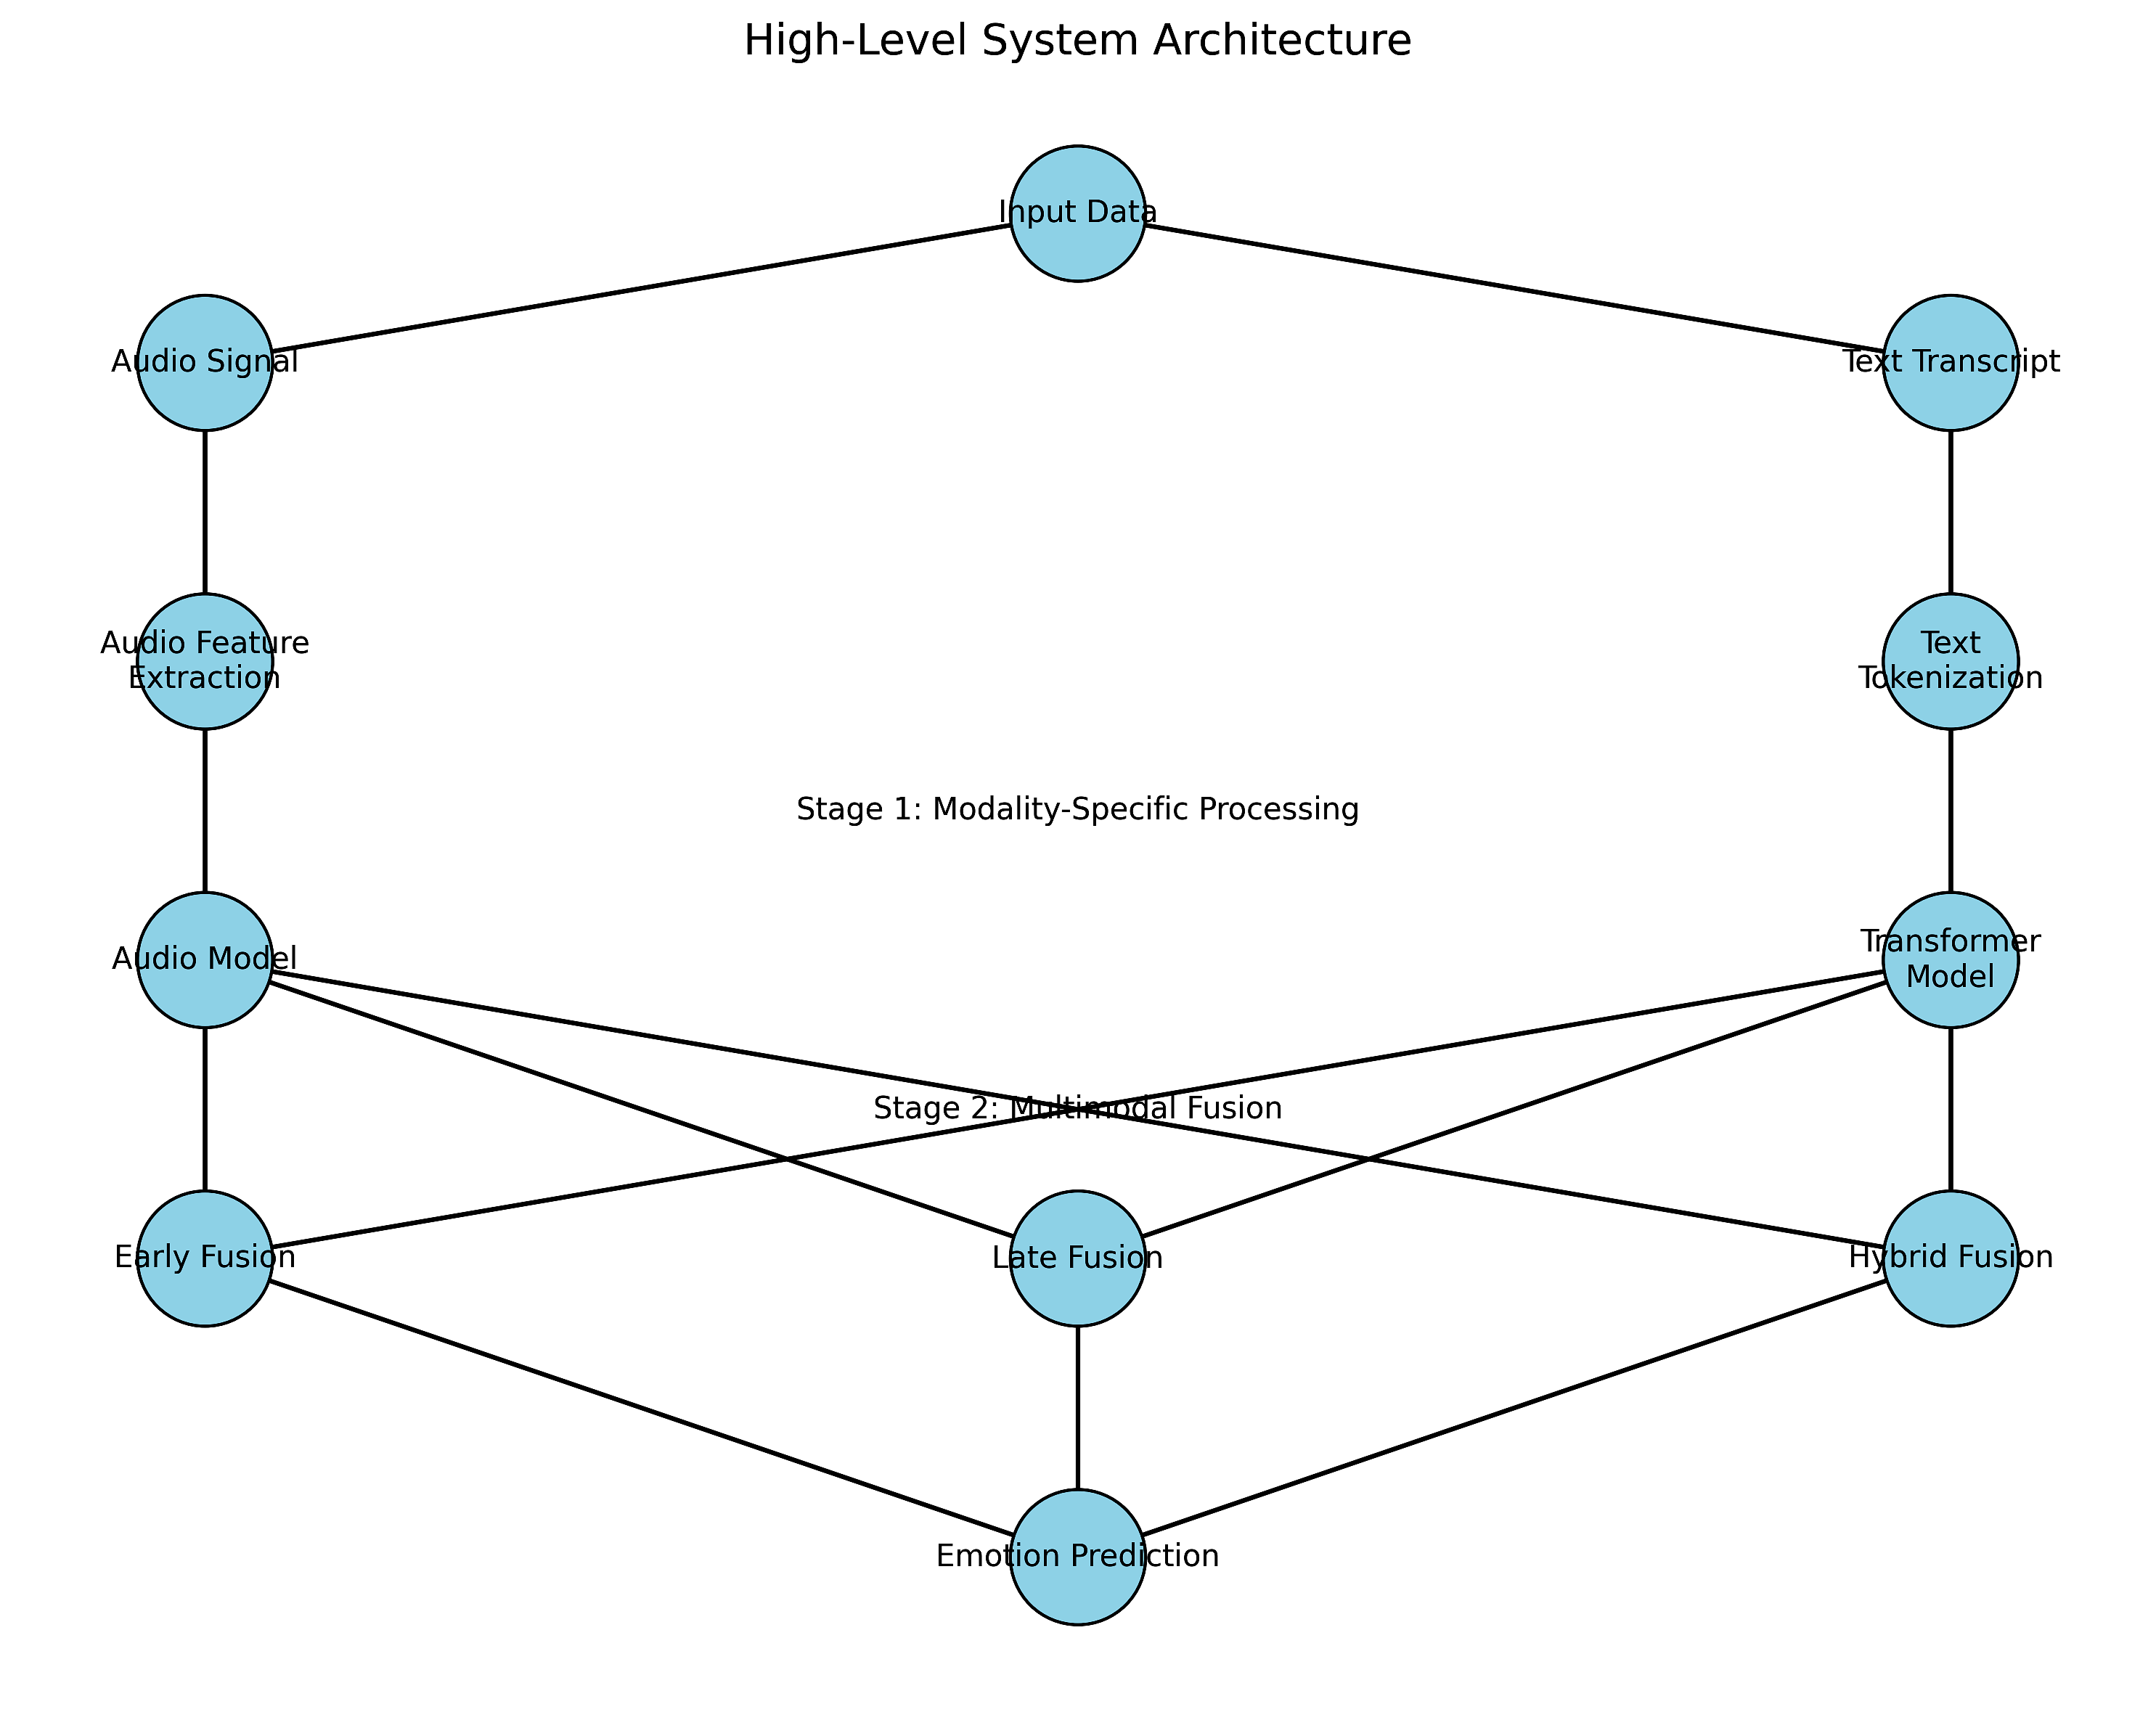
\includegraphics[width=0.5\textwidth]{figures/system_architecture.png}
\end{center}
\end{frame}

\begin{frame}
\frametitle{Evolution of Emotion Recognition}
\begin{itemize}
    \item \textbf{Pre-2012}: Mostly rule-based systems and traditional ML
    \begin{itemize}
        \item SVM, Decision Trees, Bayesian methods
        \item Handcrafted features like lexicons and acoustic parameters
    \end{itemize}
    \item \textbf{Deep Learning Era (2013-2017)}: 
    \begin{itemize}
        \item CNNs, RNNs for feature extraction
        \item Word embeddings (Word2Vec, GloVe)
    \end{itemize}
    \item \textbf{Transformer Era (2018-Present)}:
    \begin{itemize}
        \item BERT, RoBERTa, XLNet, DeBERTa
        \item Attention-based architectures enable better context modeling
    \end{itemize}
\end{itemize}
\end{frame}

\section{Methodology}

\begin{frame}
\frametitle{System Architecture}
\begin{center}
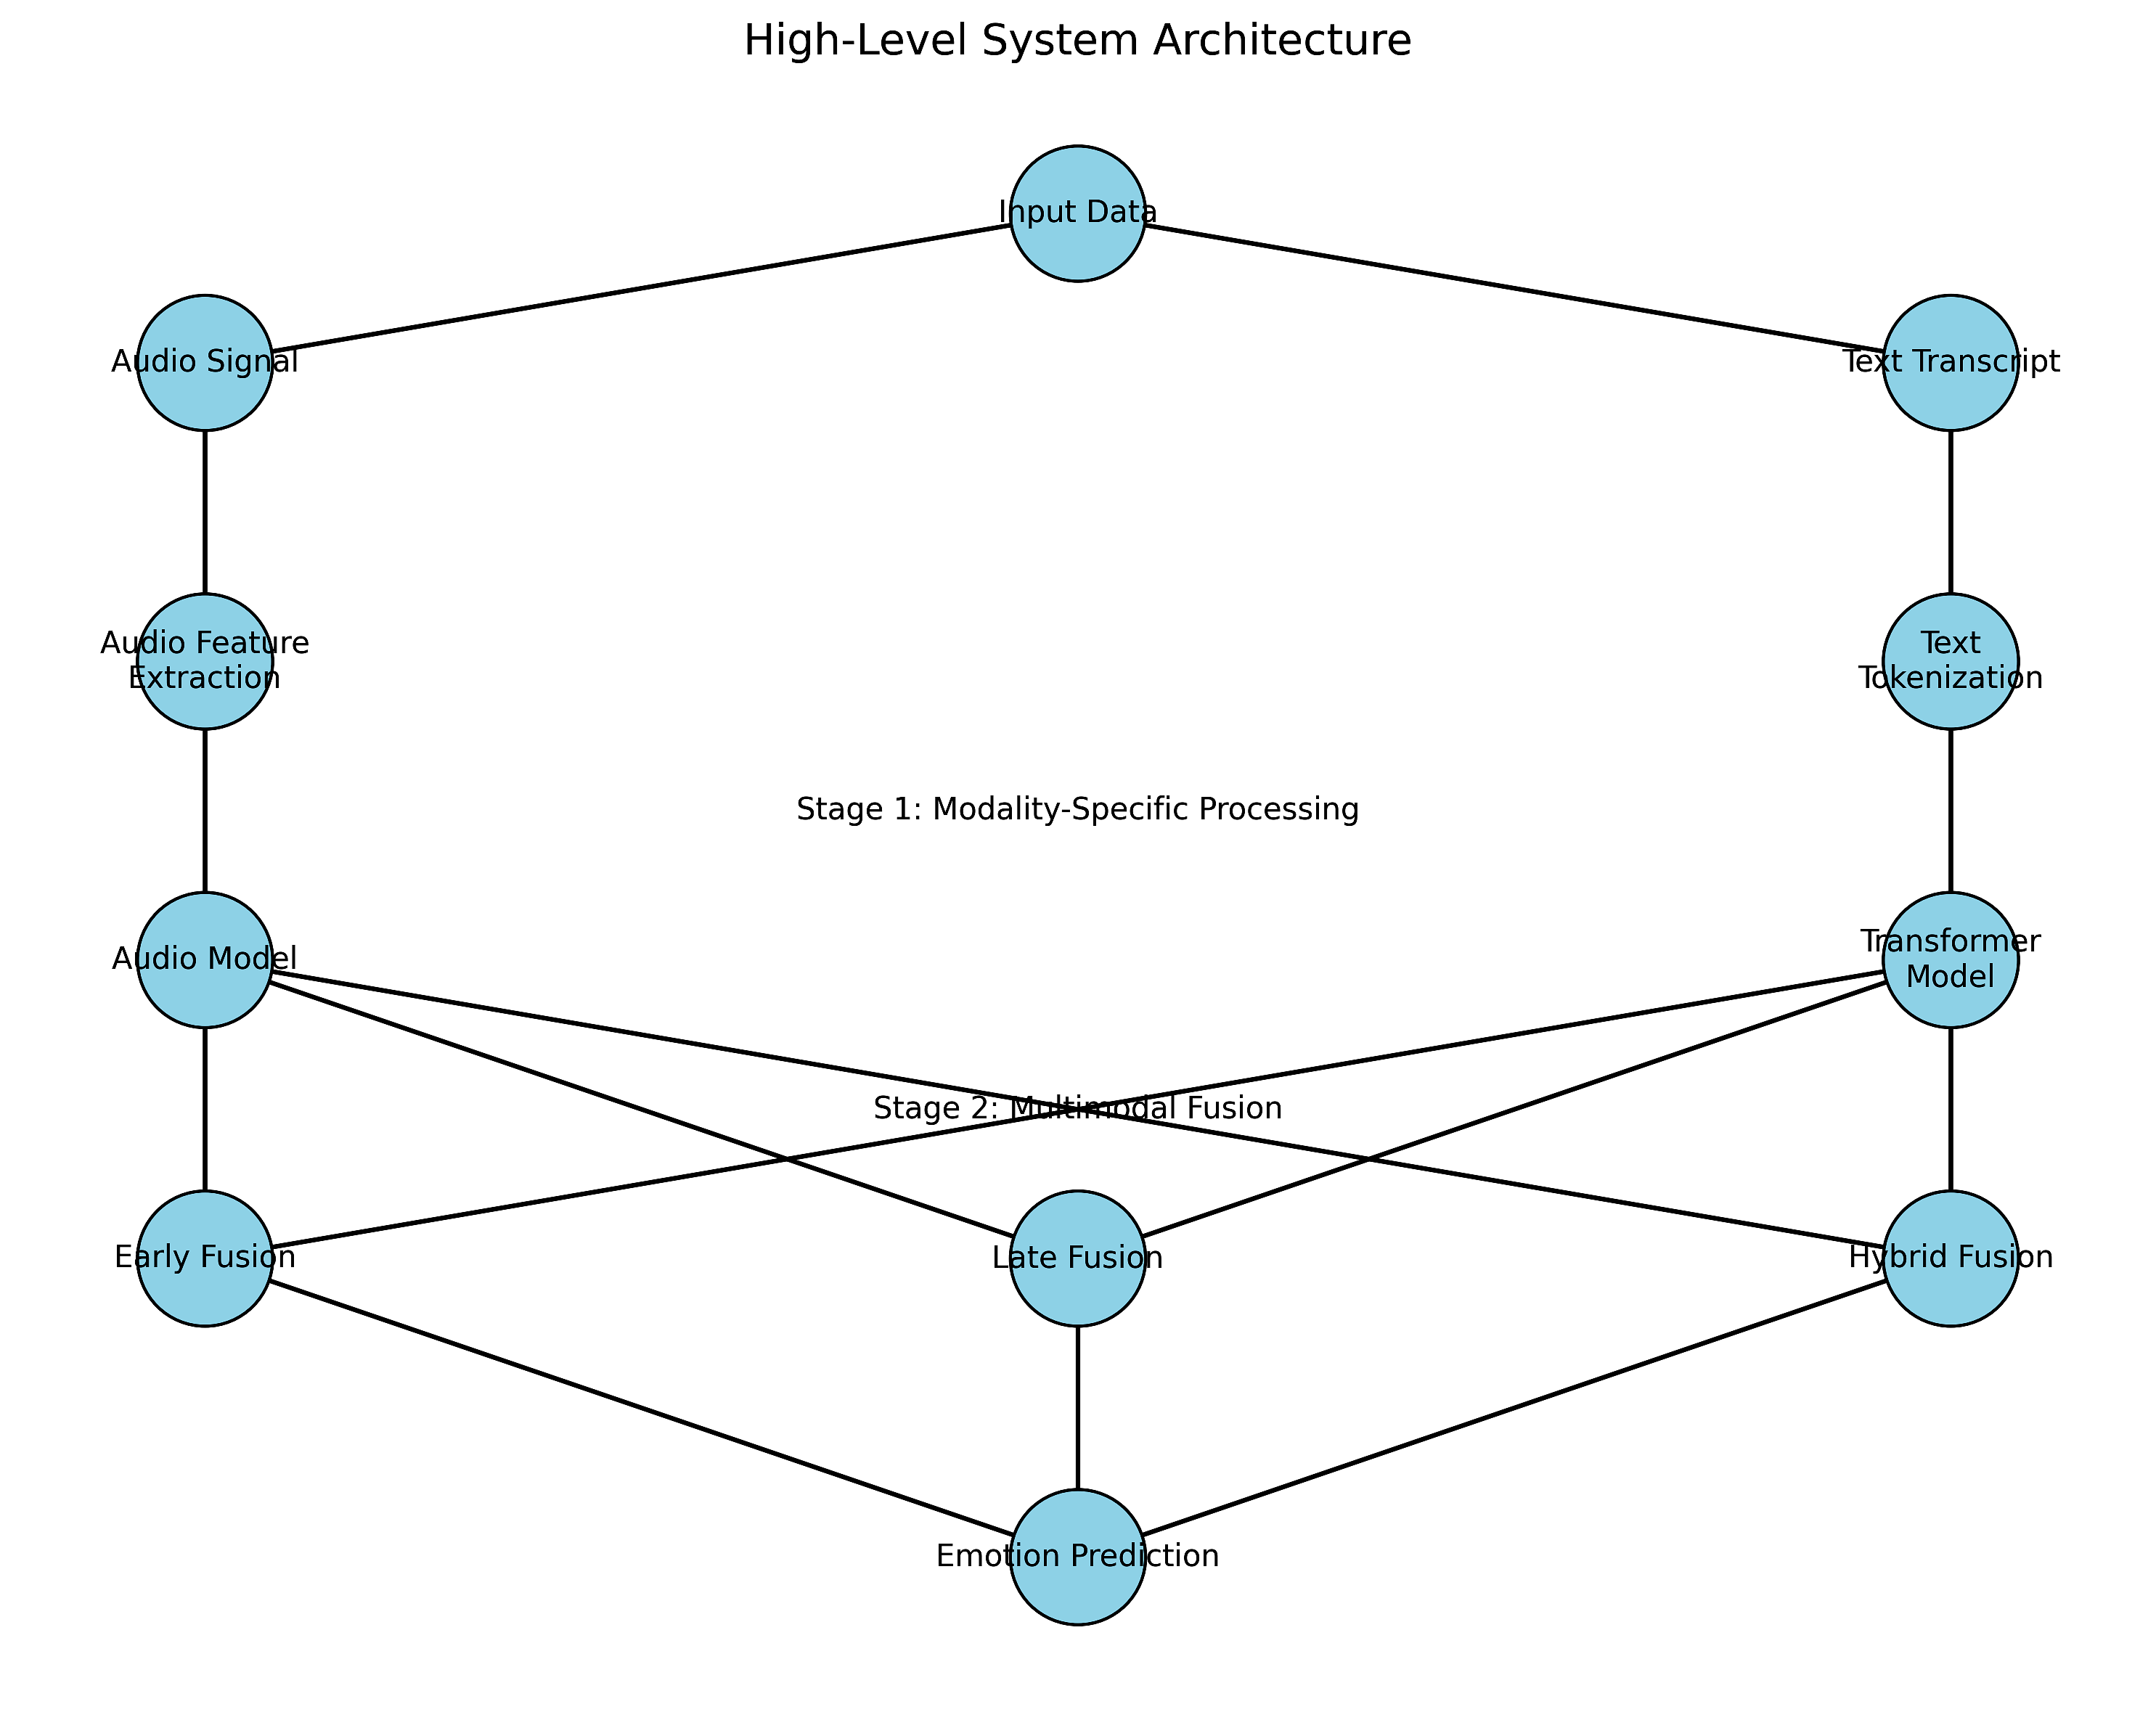
\includegraphics[width=0.9\textwidth]{figures/system_architecture.png}
\caption{Two-stage emotion detection system architecture}
\end{center}

\begin{itemize}
    \item \textbf{Stage 1}: Predict dimensional values (Arousal, Valence, Dominance)
    \item \textbf{Stage 2}: Map dimensional values to categorical emotions
\end{itemize}
\end{frame}

\begin{frame}
\frametitle{Text Processing Models}
\begin{center}
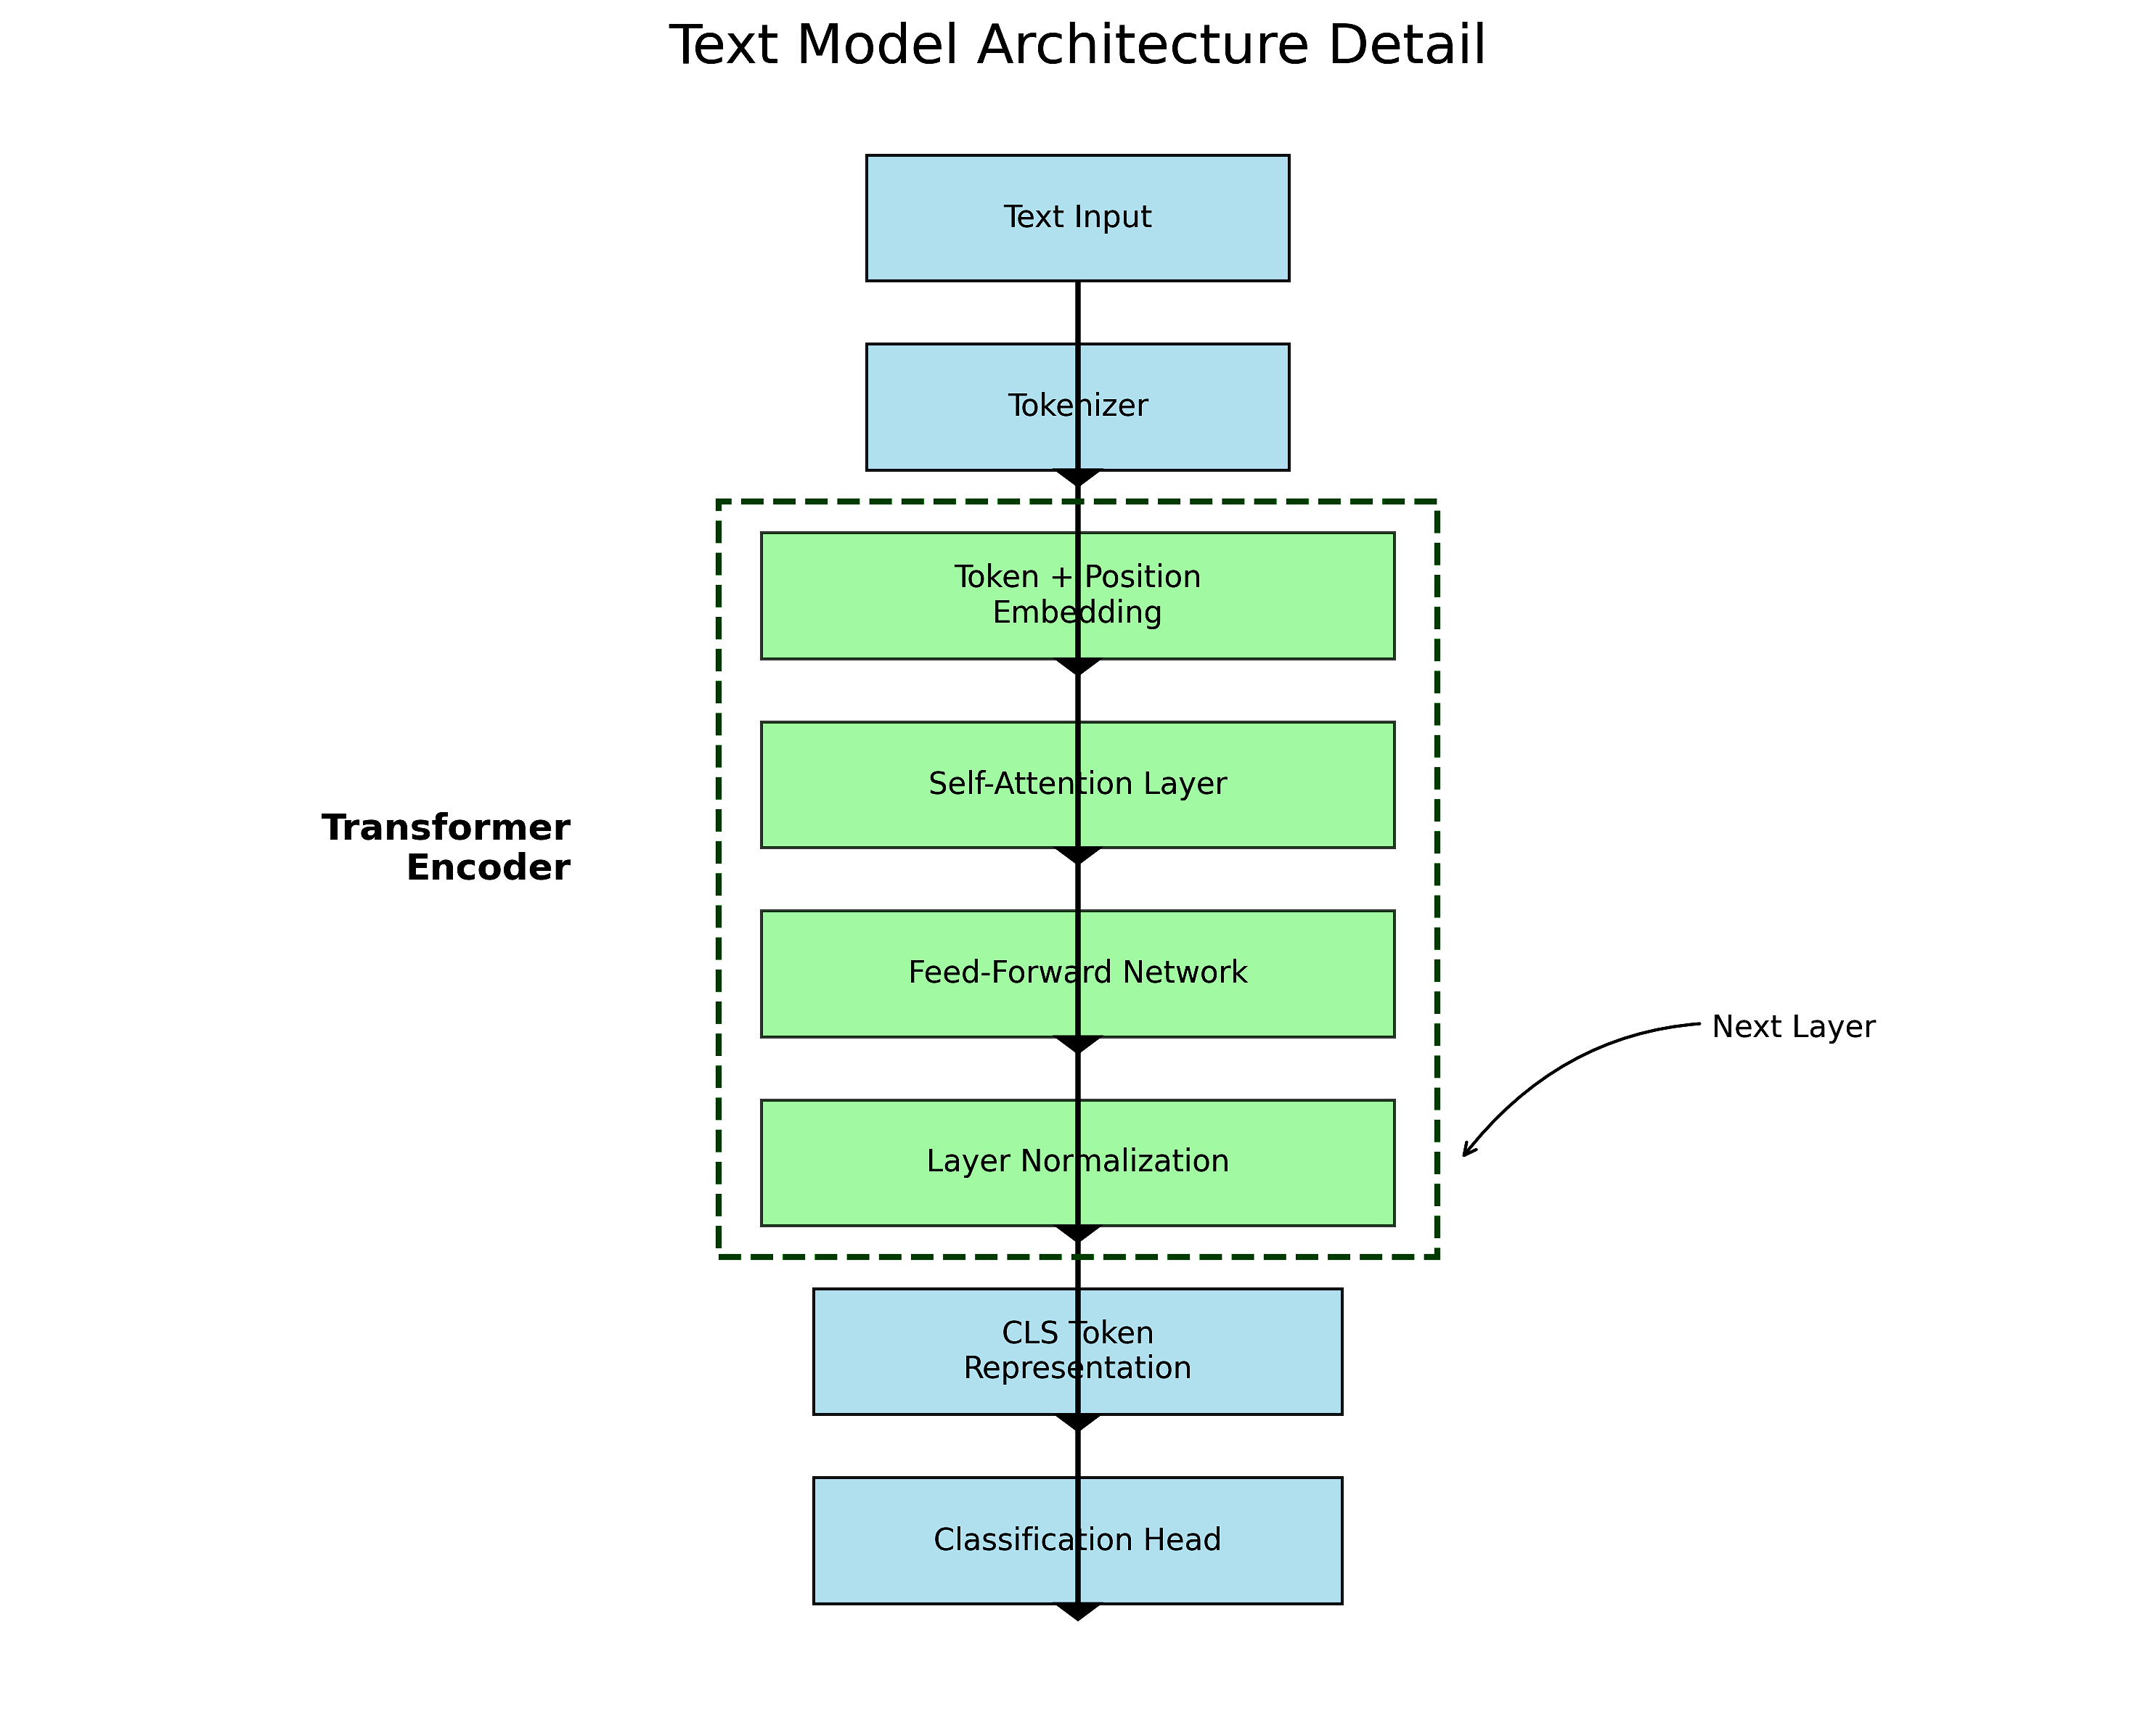
\includegraphics[width=0.9\textwidth]{figures/text_model_architecture.png}
\caption{Text processing pipeline with transformer models}
\end{center}

\begin{itemize}
    \item \textbf{BERT}: Bidirectional context modeling (110M parameters)
    \item \textbf{RoBERTa}: Optimized BERT with larger corpus (125M parameters)
    \item \textbf{XLNet}: Autoregressive pretraining
    \item \textbf{ALBERT}: Parameter-efficient BERT variant
    \item \textbf{ELECTRA}: Generator-discriminator pretraining
    \item \textbf{DeBERTa}: Disentangled attention mechanism
\end{itemize}
\end{frame}

\begin{frame}
\frametitle{Audio Feature Extraction}
\begin{center}
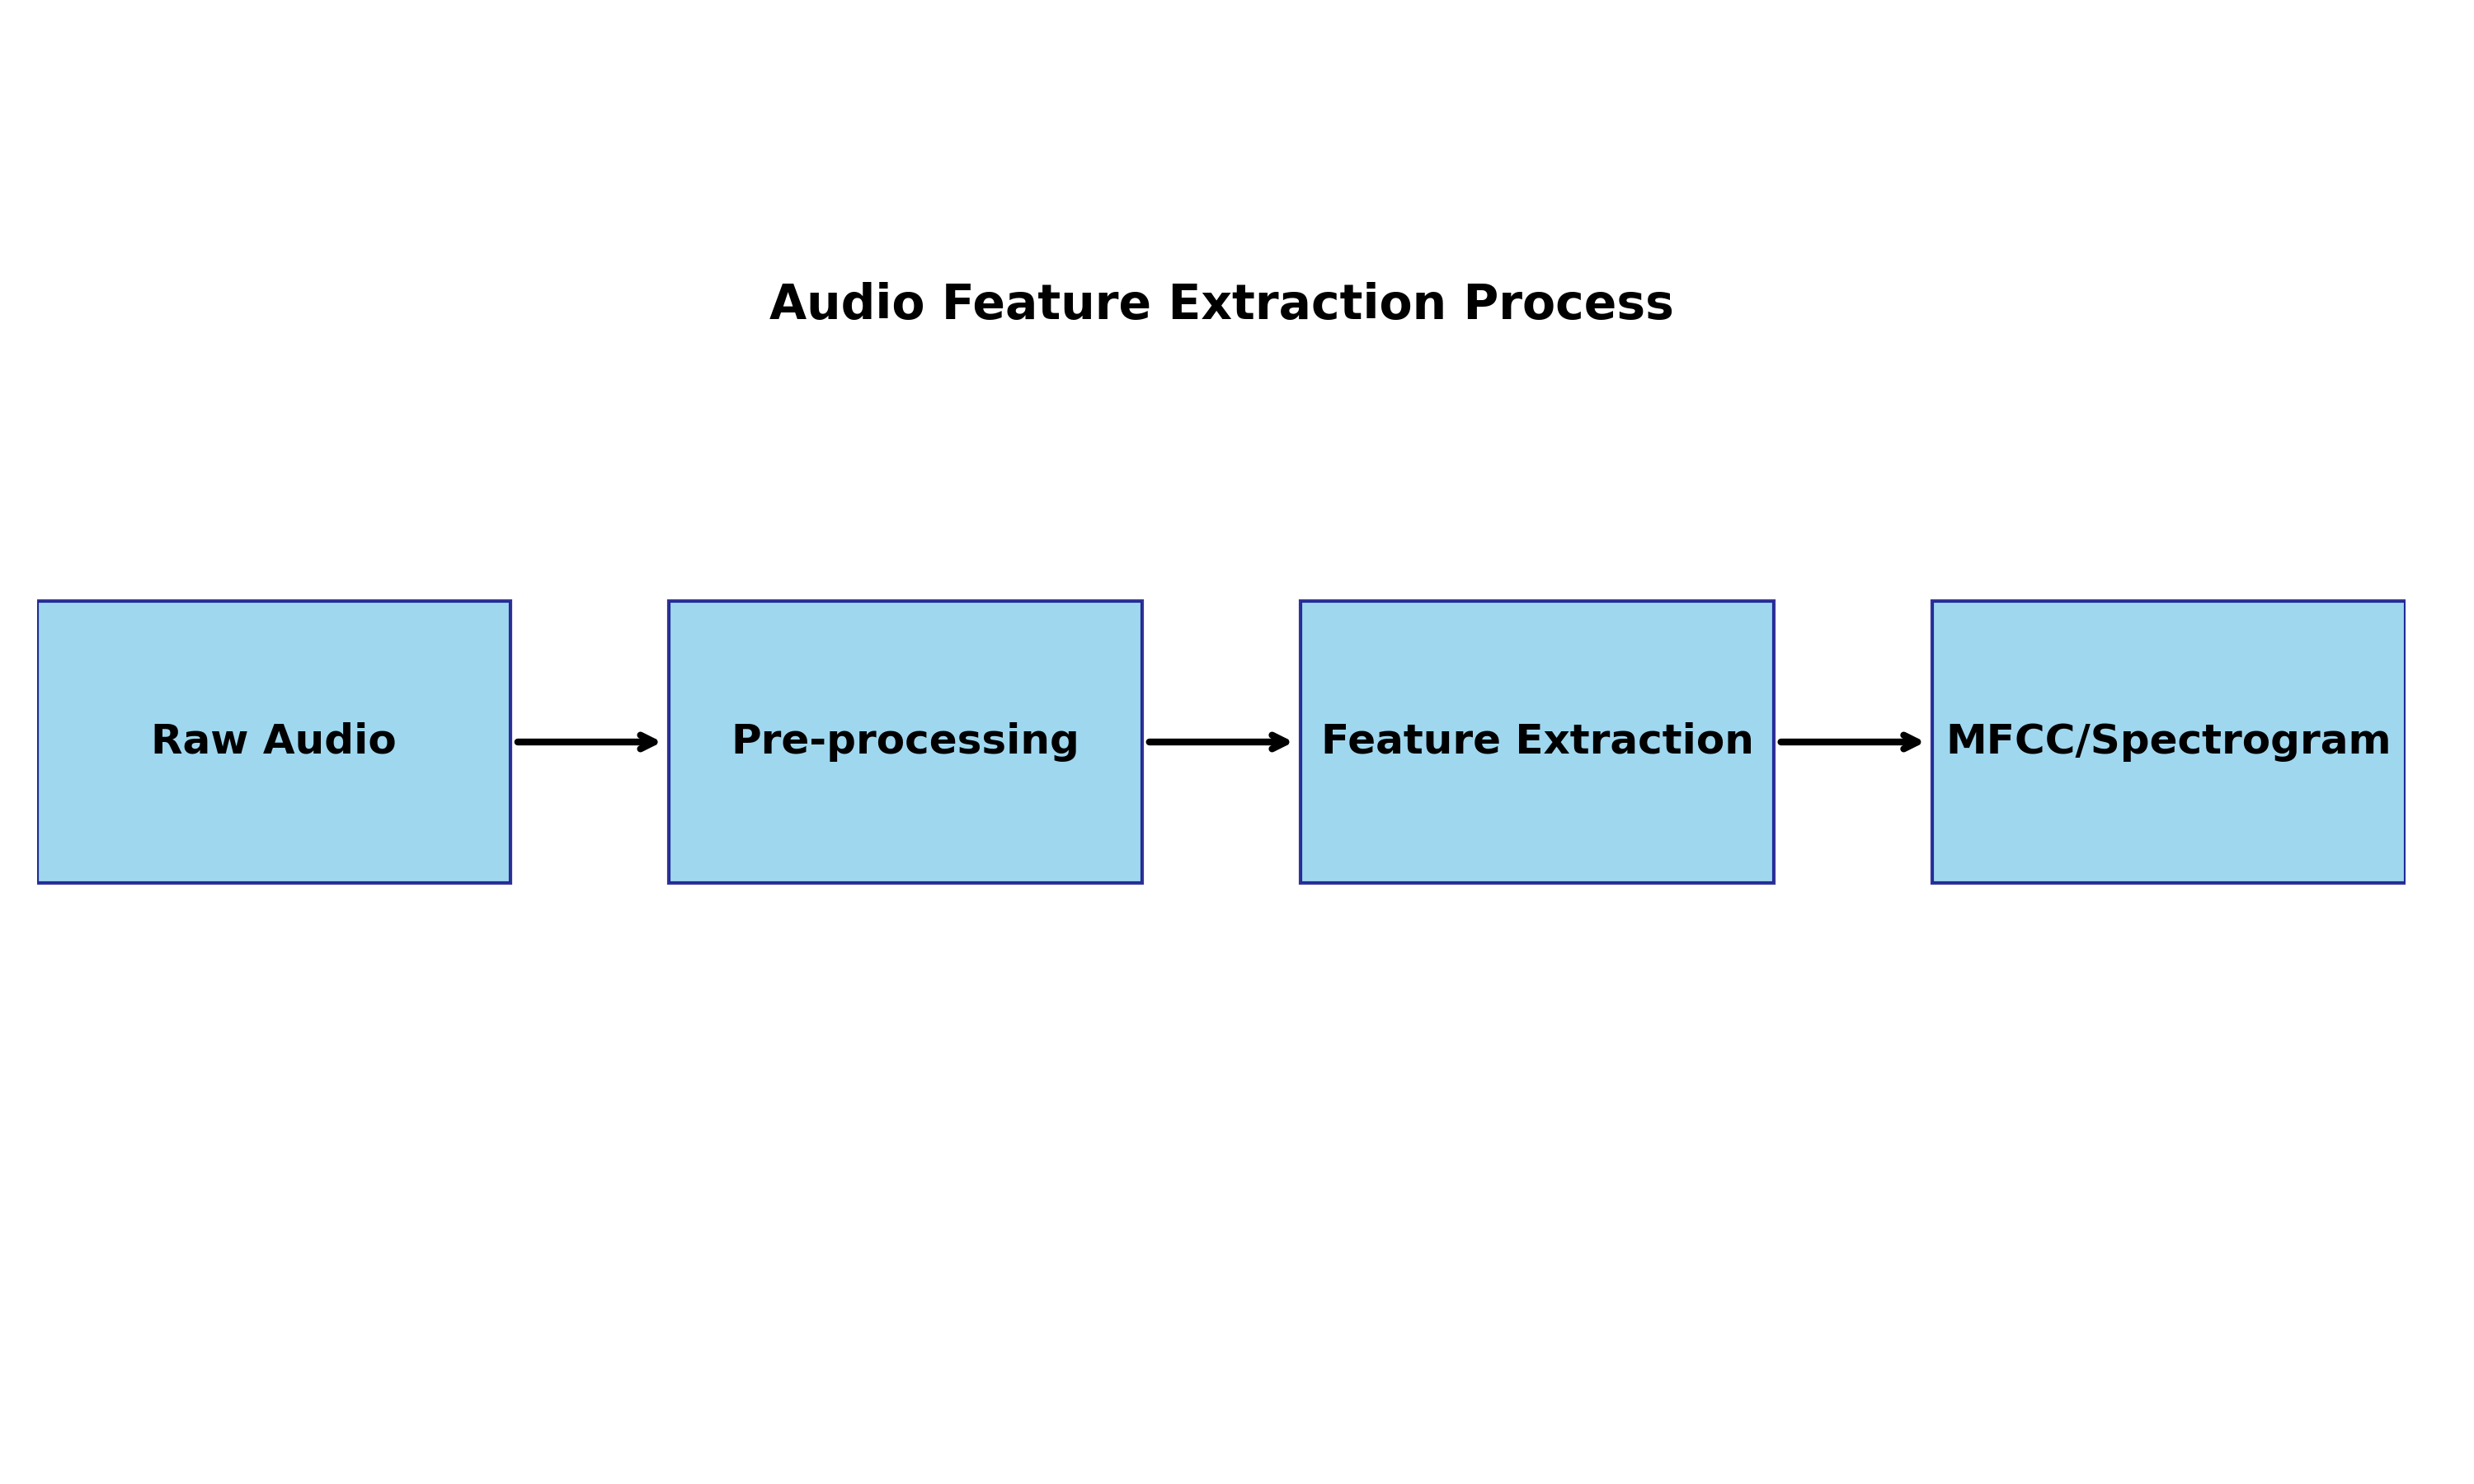
\includegraphics[width=0.9\textwidth]{figures/audio_feature_extraction.png}
\caption{Audio feature extraction pipeline}
\end{center}

\begin{itemize}
    \item \textbf{MFCCs}: Mel-Frequency Cepstral Coefficients (vocal tract characteristics)
    \item \textbf{Spectrograms}: Visual representation of spectrum of frequencies
    \item \textbf{Prosodic Features}: Pitch, energy, speaking rate, rhythm
    \item \textbf{Wav2vec Embeddings}: Self-supervised audio representations
\end{itemize}
\end{frame}

\begin{frame}
\frametitle{Fusion Strategies}
\begin{center}
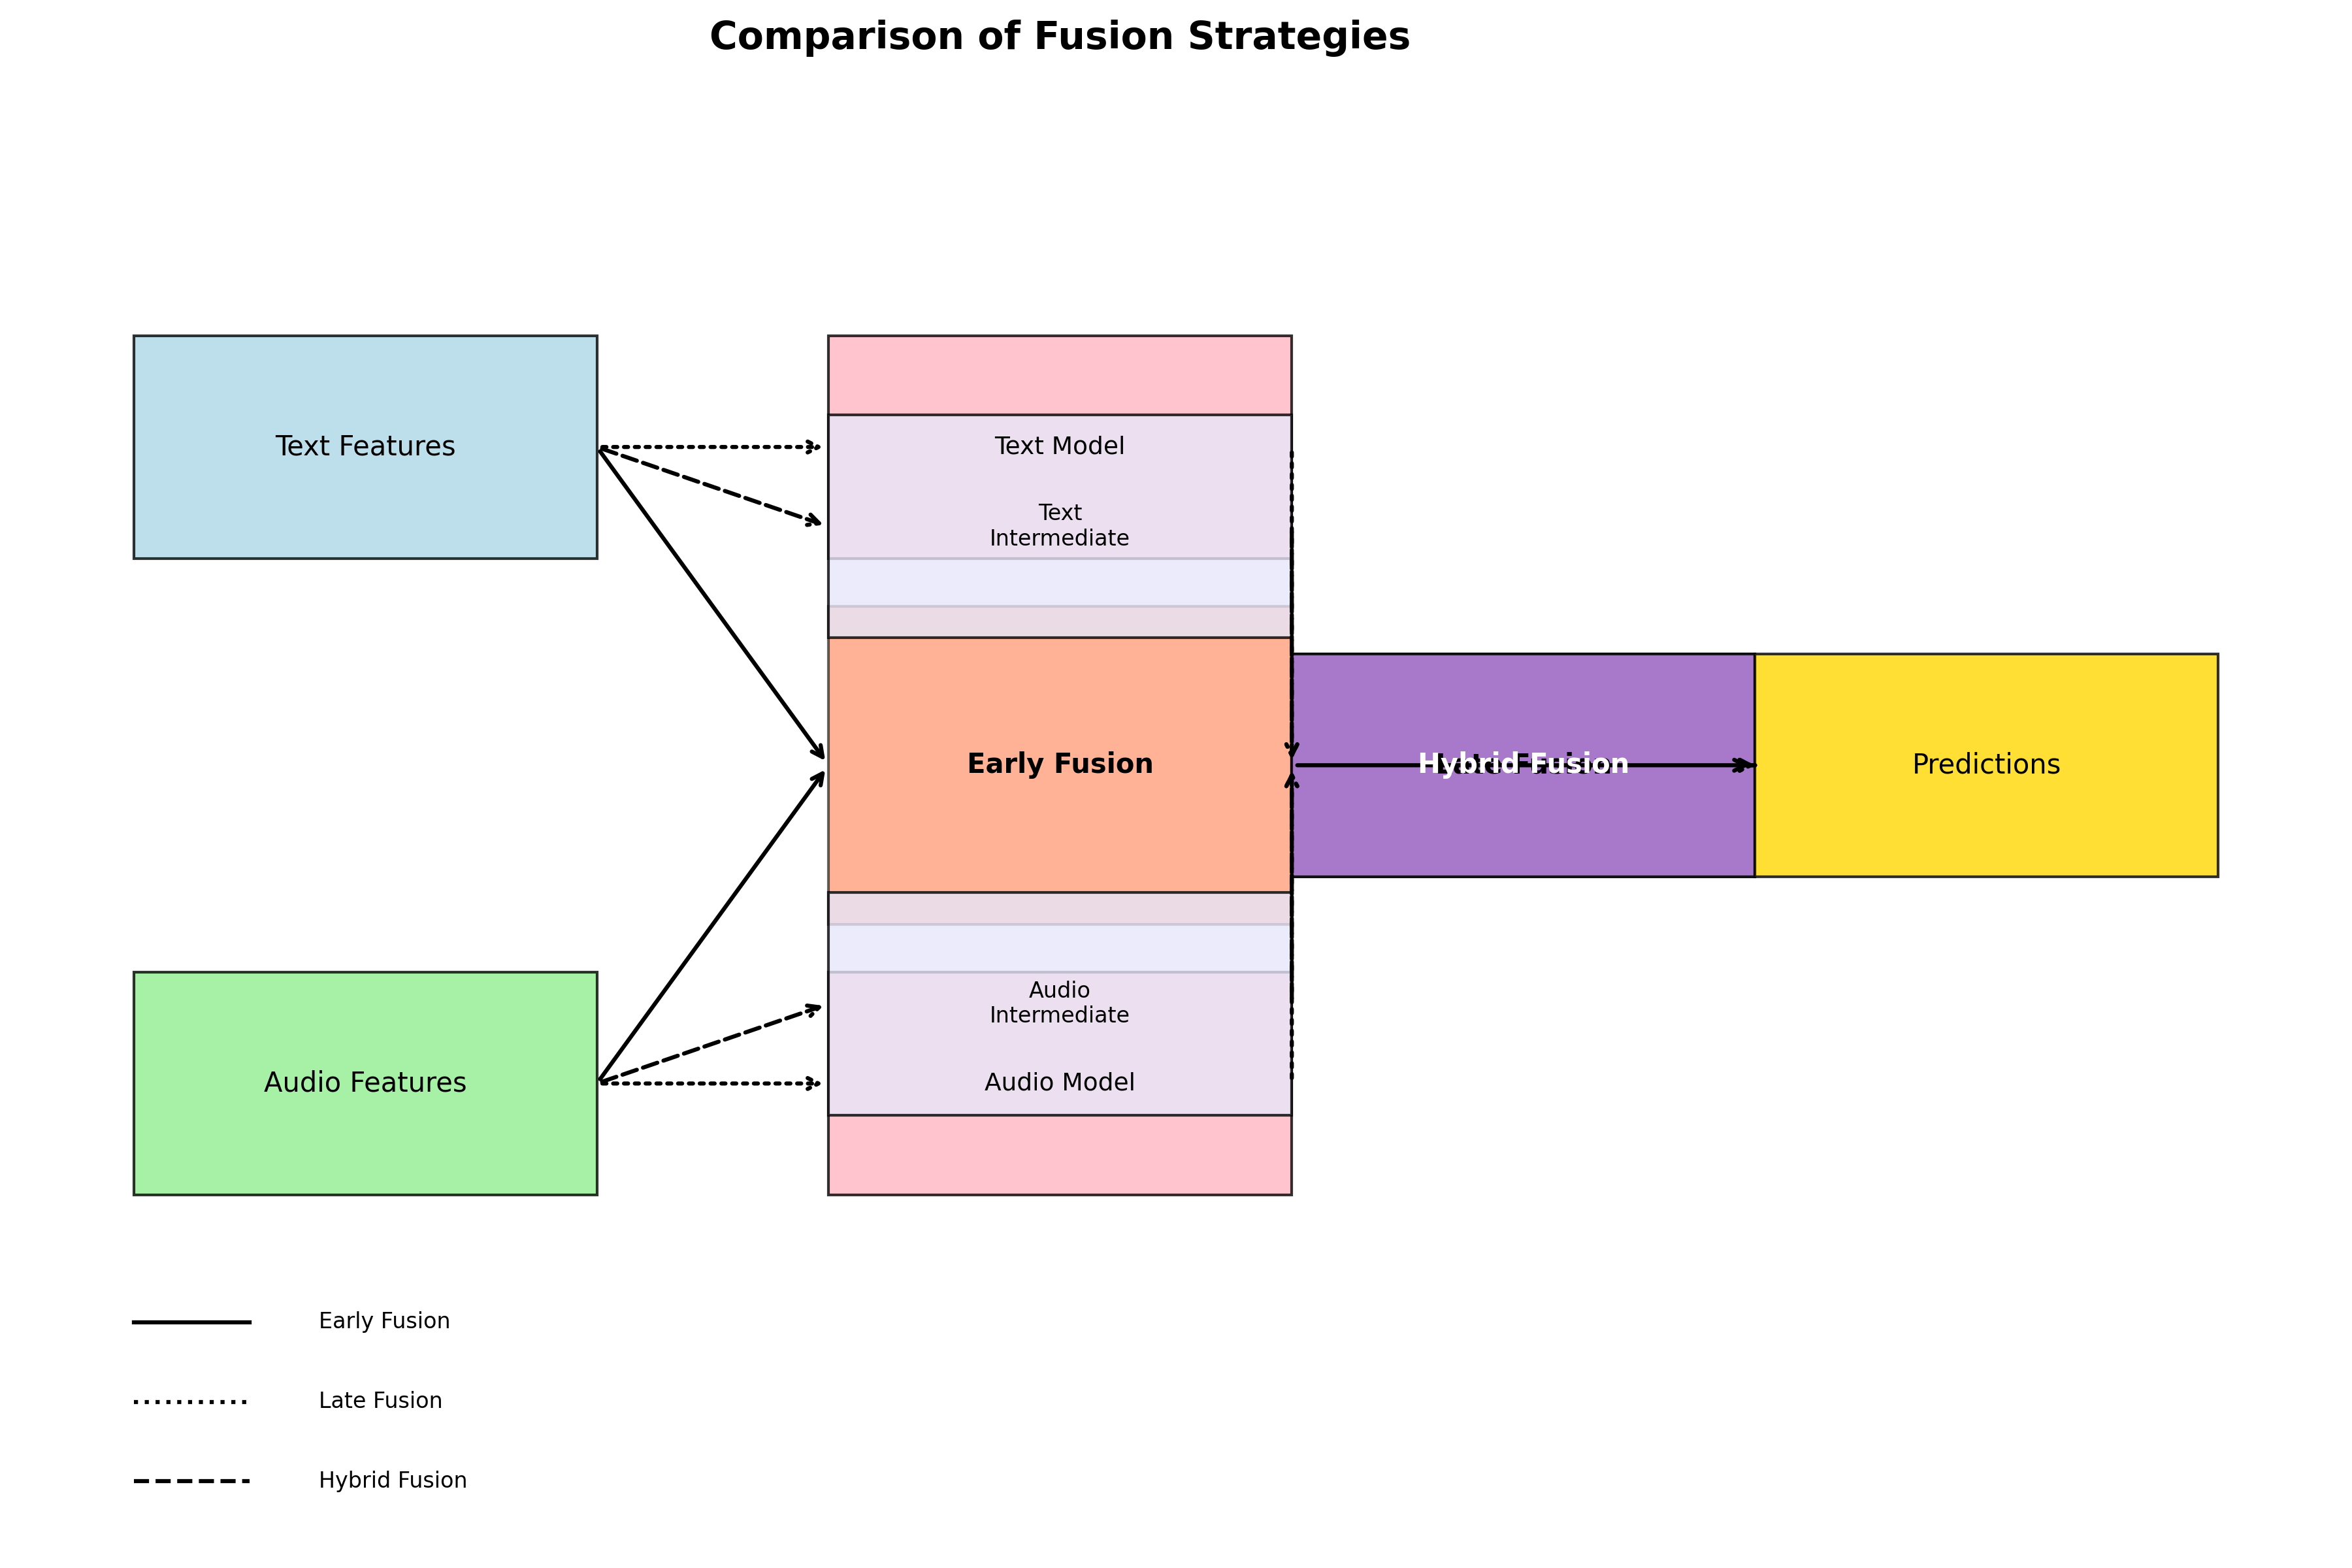
\includegraphics[width=0.9\textwidth]{figures/fusion_strategies.png}
\caption{Multimodal fusion approaches}
\end{center}

\begin{itemize}
    \item \textbf{Early Fusion}: Combine raw features before processing
    \item \textbf{Late Fusion}: Process modalities independently, combine predictions
    \item \textbf{Hybrid Fusion}: Combine at intermediate processing stages
    \item \textbf{Attention-Based Fusion}: Dynamic weighting based on importance
\end{itemize}
\end{frame}

\begin{frame}
\frametitle{Experimental Setup}
\begin{itemize}
    \item \textbf{Dataset}: IEMOCAP (Interactive Emotional Dyadic Motion Capture)
    \begin{itemize}
        \item 12 hours of audio-visual data
        \item 10 speakers (5 male, 5 female)
        \item Both categorical and dimensional annotations
    \end{itemize}
    \item \textbf{Implementation}: PyTorch, Hugging Face Transformers
    \item \textbf{Training Protocol}:
    \begin{itemize}
        \item AdamW optimizer with linear learning rate schedule
        \item Early stopping based on validation loss
        \item 5-fold cross-validation
    \end{itemize}
    \item \textbf{Evaluation Metrics}: Accuracy, F1 (Macro/Micro), RMSE, MAE
\end{itemize}
\end{frame}

\section{Results}

\begin{frame}
\frametitle{Dimensional Emotion Prediction (Stage 1)}
\begin{center}
\begin{tabular}{|l|c|c|c|c|}
\hline
\textbf{Model} & \textbf{Modality} & \textbf{Dimension} & \textbf{Test RMSE} & \textbf{MAE} \\
\hline
RoBERTa & Text & Valence & 0.630 & 0.500 \\
         &      & Arousal & 0.730 & 0.560 \\
         &      & Dominance & 0.680 & 0.530 \\
\hline
CNN+MFCC & Audio & Valence & 0.720 & 0.590 \\
          &       & Arousal & 0.650 & 0.510 \\
          &       & Dominance & 0.700 & 0.560 \\
\hline
RoBERTa+MFCC & Multimodal & Valence & 0.610 & 0.490 \\
              &            & Arousal & 0.640 & 0.500 \\
              &            & Dominance & 0.660 & 0.520 \\
\hline
\end{tabular}
\end{center}

\begin{itemize}
    \item Text models perform better for \textbf{Valence} (positive/negative sentiment)
    \item Audio models perform better for \textbf{Arousal} (intensity/energy)
    \item Multimodal approaches show balanced performance across dimensions
\end{itemize}
\end{frame}

\begin{frame}
\frametitle{Categorical Emotion Classification}
\begin{center}
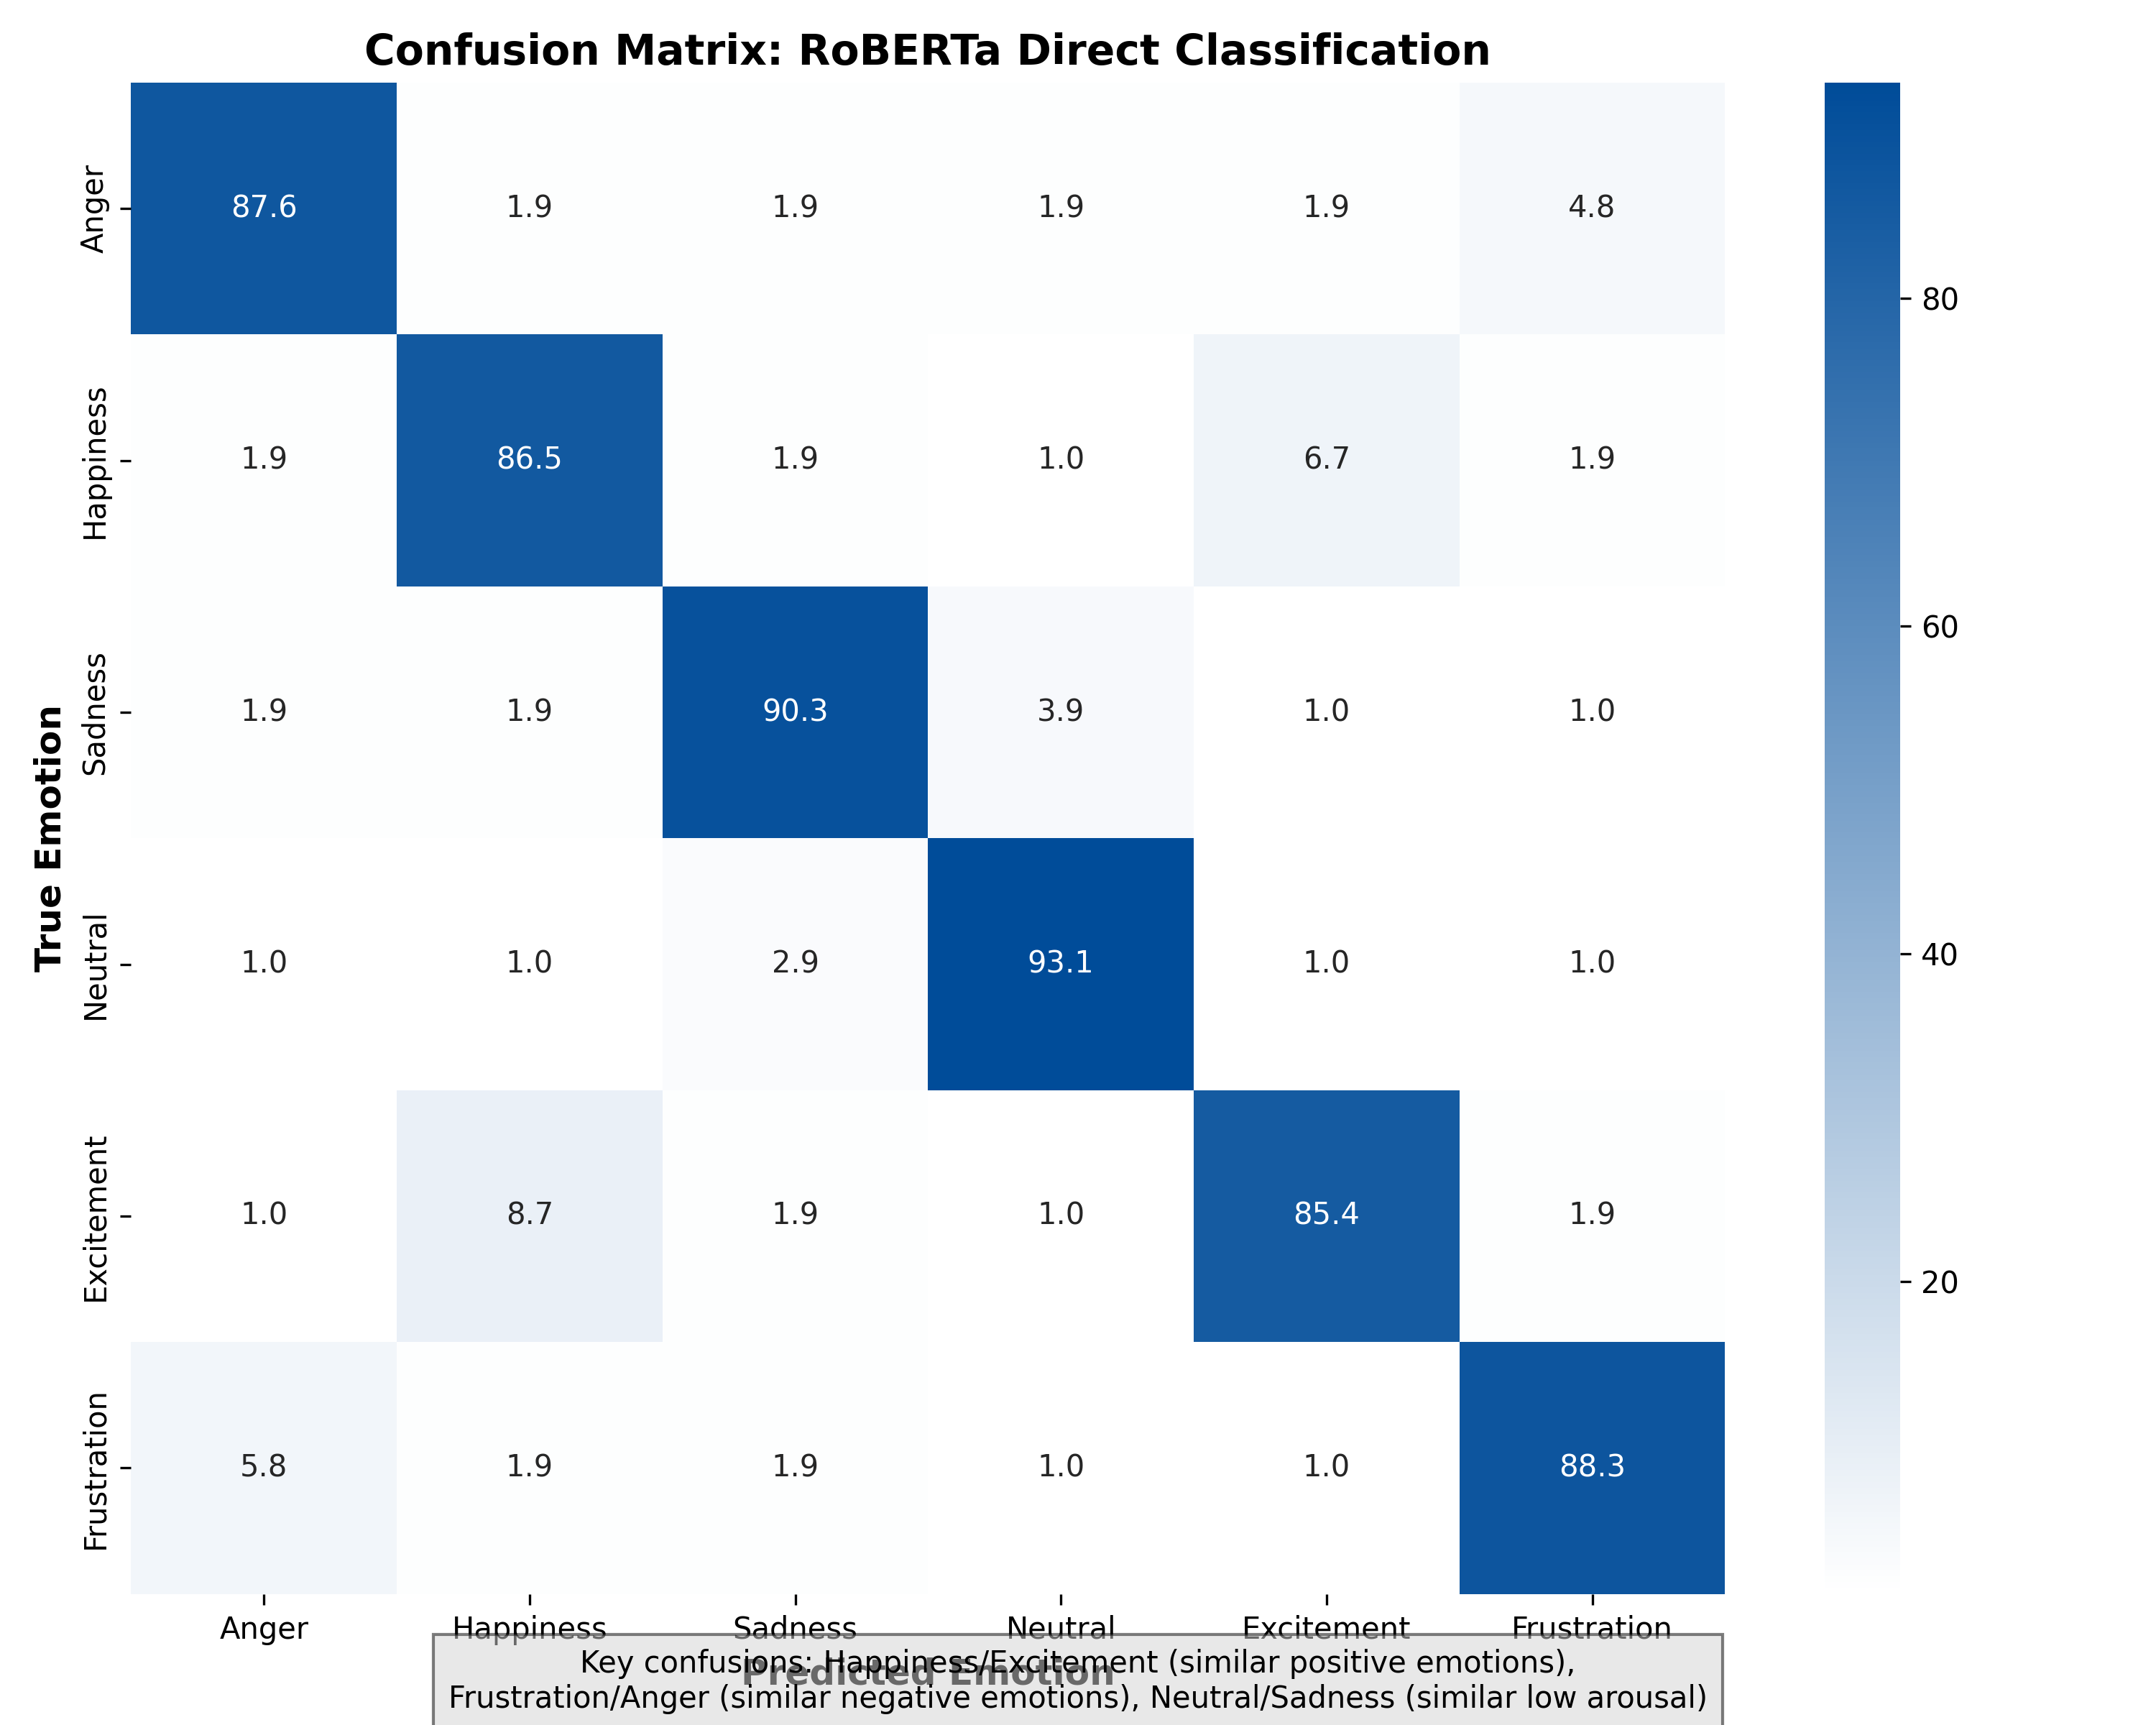
\includegraphics[width=0.9\textwidth]{figures/confusion_matrix.png}
\caption{Confusion matrix for emotion classification using RoBERTa}
\end{center}
\end{frame}

\begin{frame}
\frametitle{Two-Stage vs. Direct Classification}
\begin{center}
\begin{tabular}{|l|c|c|c|c|}
\hline
\textbf{Approach} & \textbf{Modality} & \textbf{Test Acc.} & \textbf{Macro F1} & \textbf{Micro F1} \\
\hline
Direct (RoBERTa) & Text & 0.95 & 0.94 & 0.95 \\
Two-Stage (RoBERTa) & Text & 0.92 & 0.91 & 0.92 \\
\hline
Direct (CNN+MFCC) & Audio & 0.89 & 0.87 & 0.89 \\
Two-Stage (CNN+MFCC) & Audio & 0.87 & 0.85 & 0.87 \\
\hline
Direct (RoBERTa+MFCC) & Multimodal & 0.94 & 0.93 & 0.94 \\
Two-Stage (RoBERTa+MFCC) & Multimodal & 0.90 & 0.89 & 0.90 \\
\hline
\end{tabular}
\end{center}

\begin{itemize}
    \item Direct classification consistently outperforms two-stage approach
    \item But two-stage approach provides richer emotional representation
    \item Performance gap consistent across modalities (1.5-2.5\%)
\end{itemize}
\end{frame}

\begin{frame}
\frametitle{Modality Importance}
\begin{center}
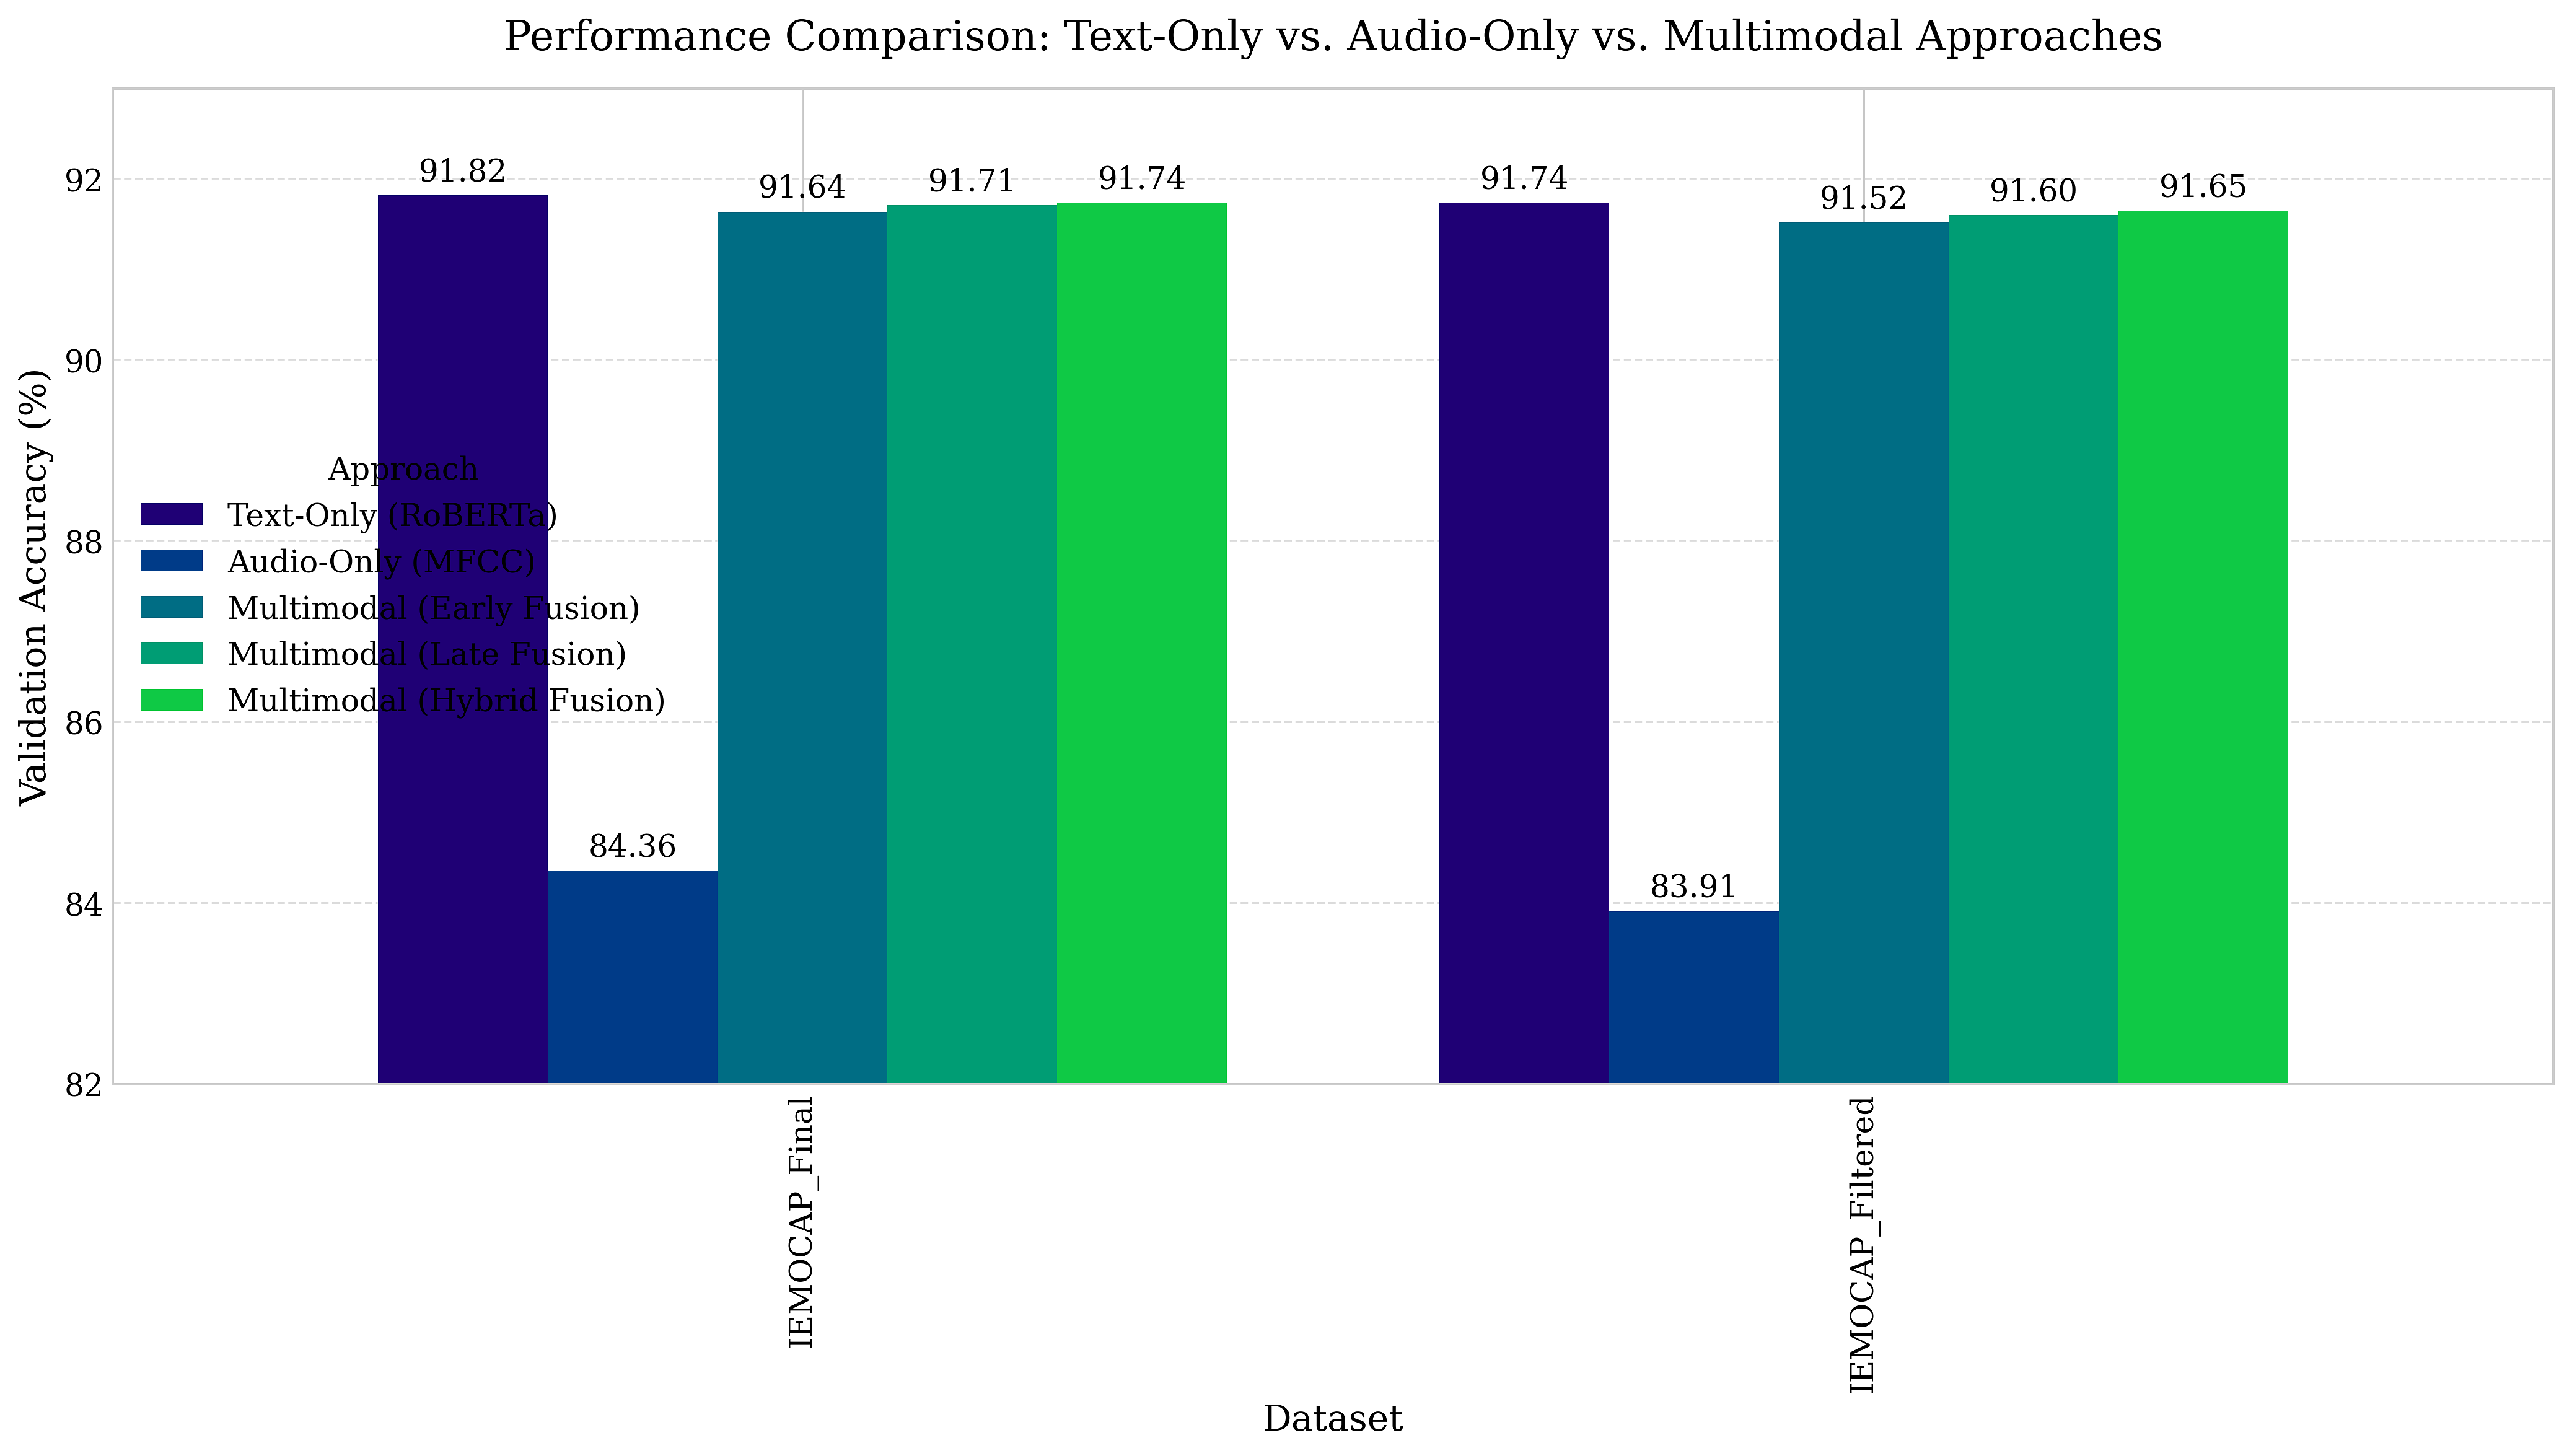
\includegraphics[width=0.9\textwidth]{figures/modality_comparison.png}
\caption{Performance comparison across modalities}
\end{center}

\begin{itemize}
    \item Text-only approaches slightly outperform multimodal approaches
    \item But gap narrows with optimal fusion strategies
    \item Audio-only models lag but provide complementary information
\end{itemize}
\end{frame}

\begin{frame}
\frametitle{Transformer Model Comparison}
\begin{center}
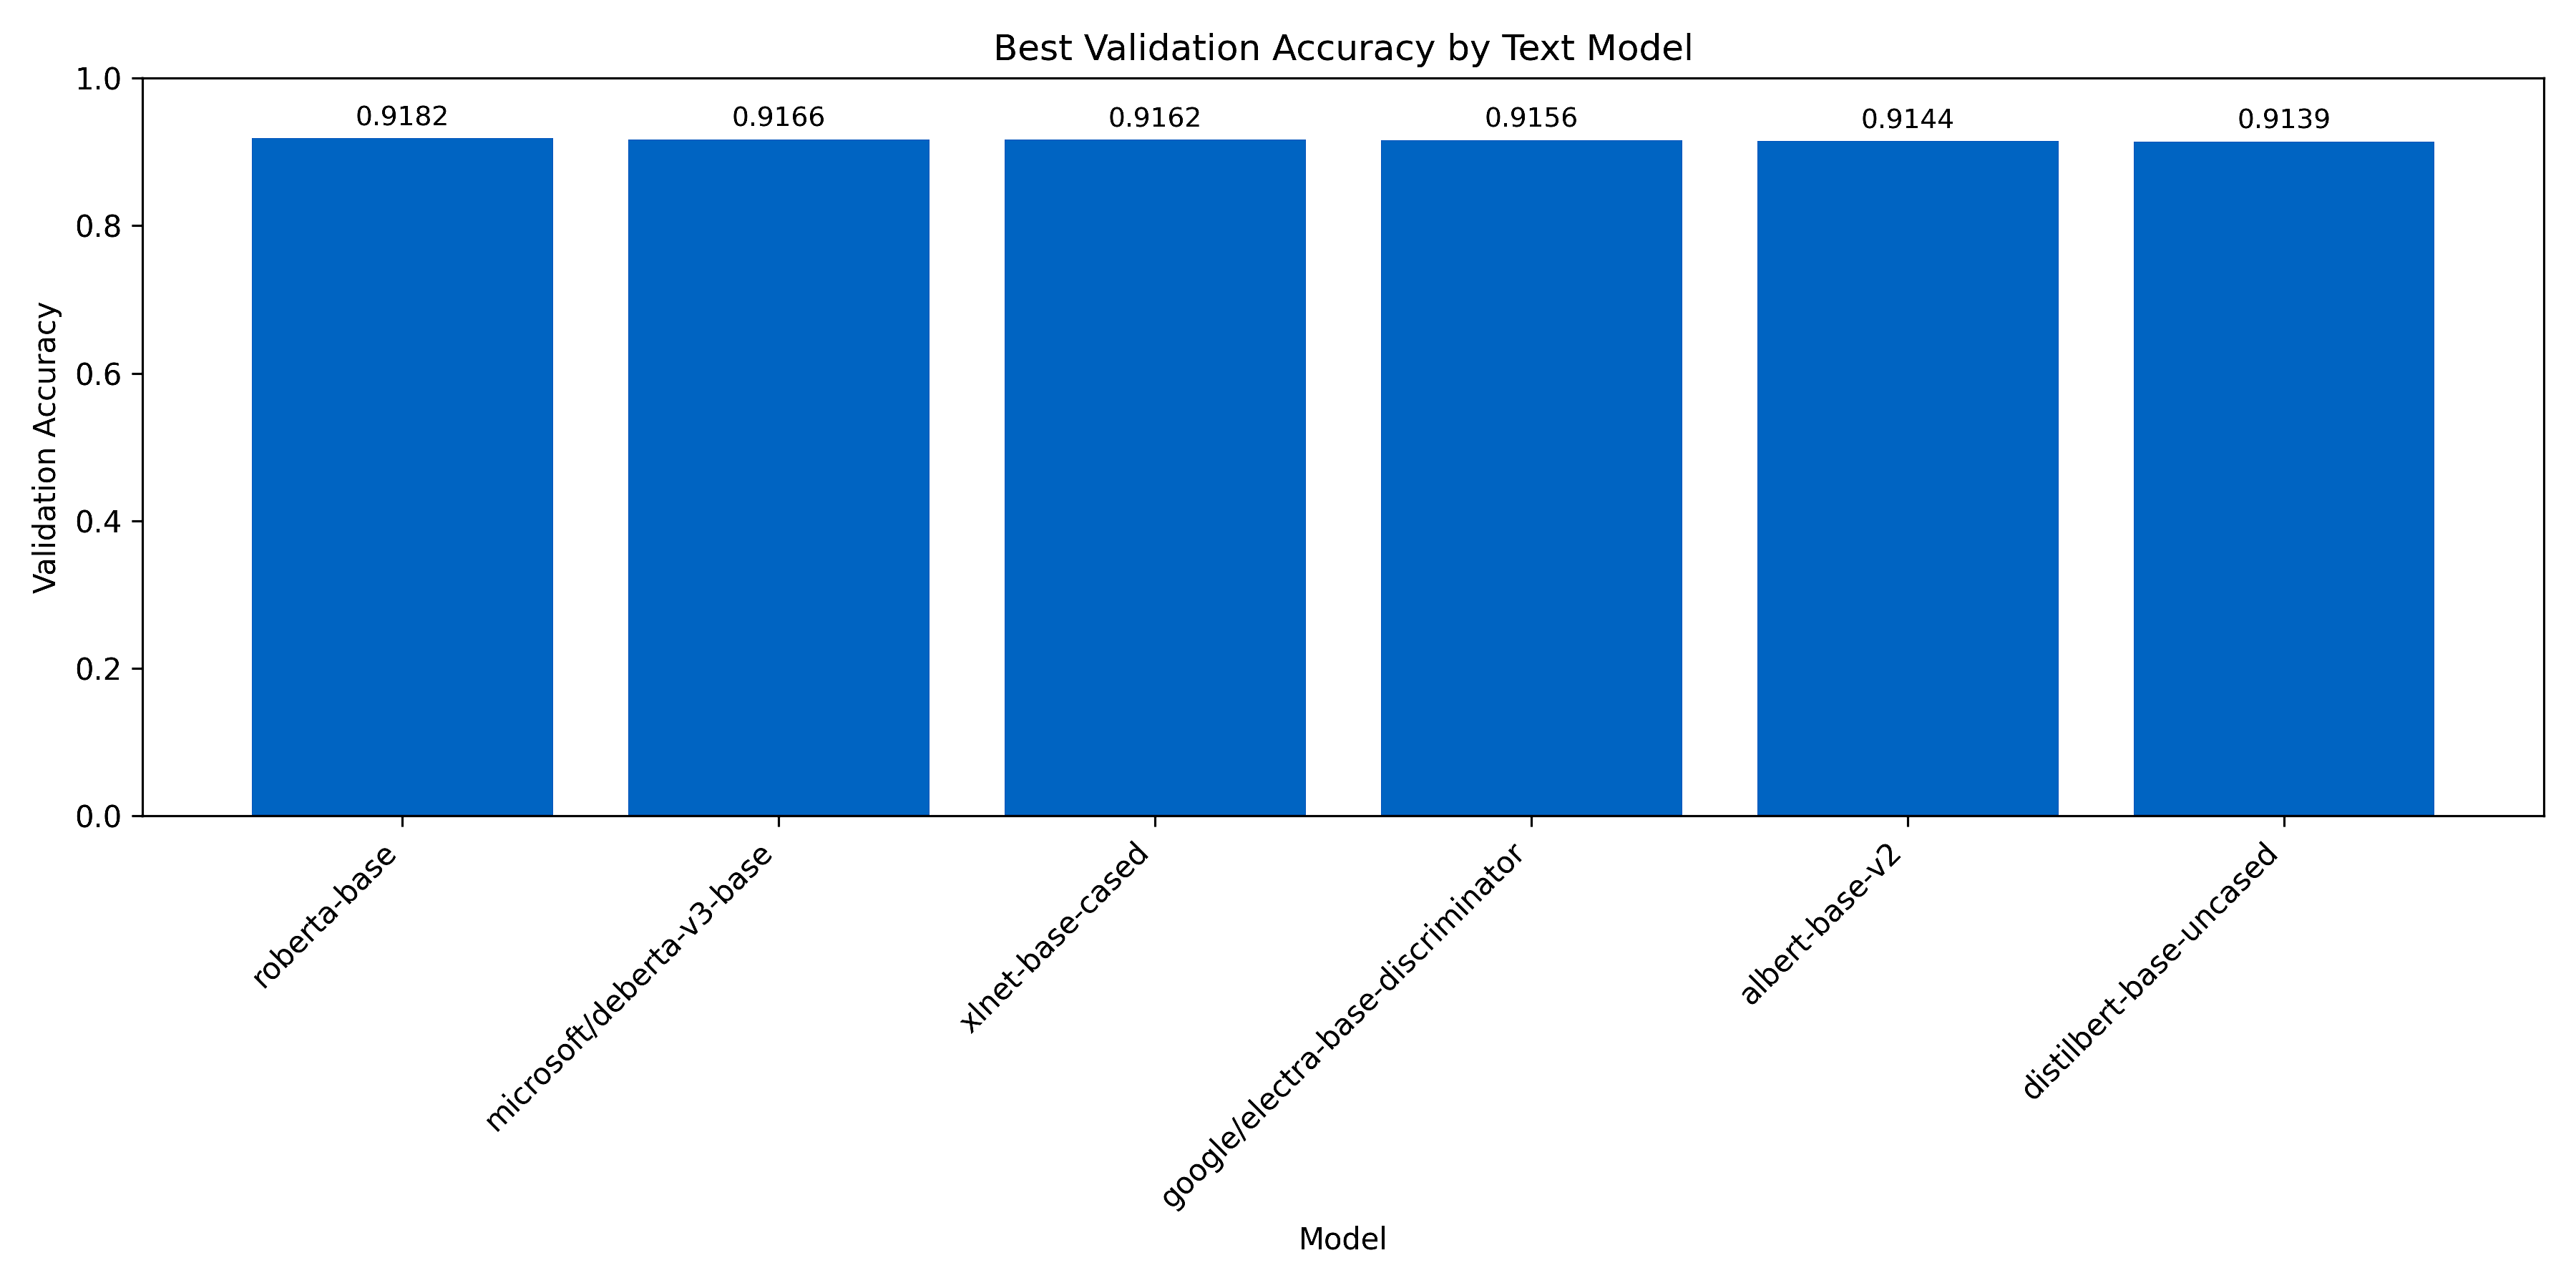
\includegraphics[width=0.9\textwidth]{figures/text_model_comparison.png}
\caption{Performance comparison of transformer models}
\end{center}

\begin{itemize}
    \item RoBERTa consistently outperforms other models
    \item DeBERTa shows strong performance, particularly for valence
    \item ALBERT shows lowest performance despite parameter efficiency
\end{itemize}
\end{frame}

\begin{frame}
\frametitle{Audio Feature Effectiveness}
\begin{center}
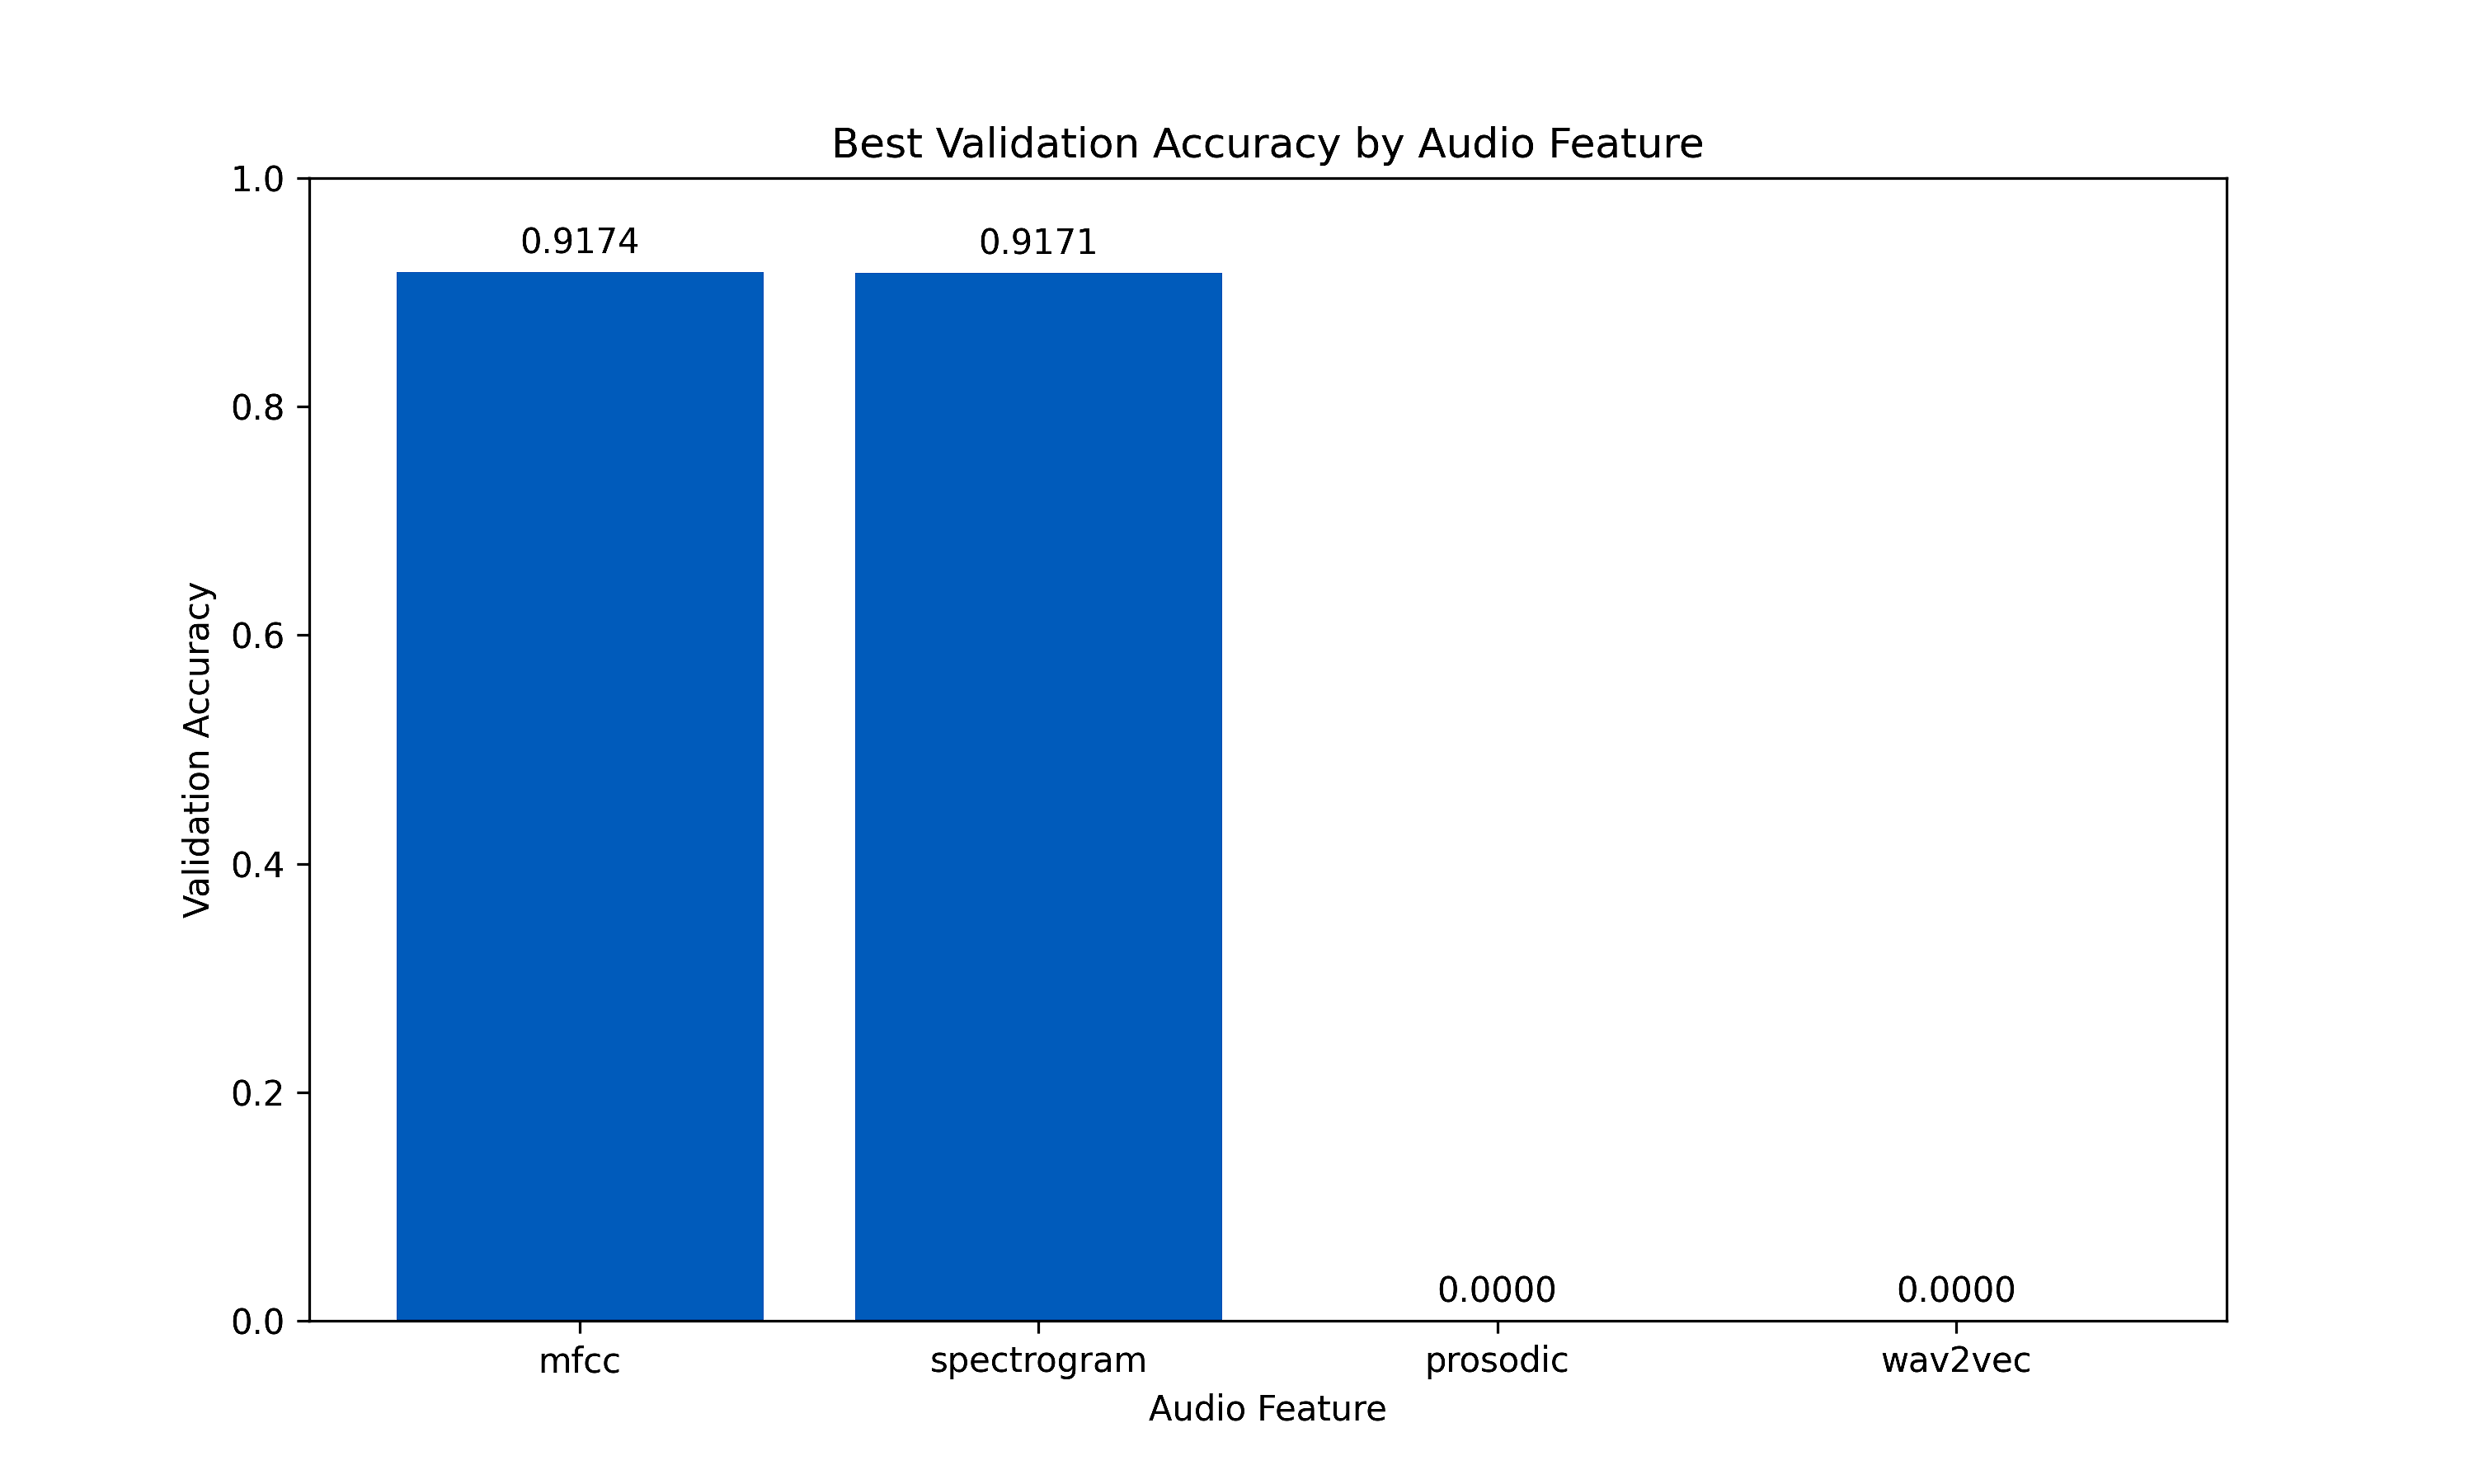
\includegraphics[width=0.9\textwidth]{figures/audio_feature_comparison.png}
\caption{Comparison of audio feature extraction methods}
\end{center}

\begin{itemize}
    \item MFCCs provide the best performance for emotion detection
    \item Spectrograms capture more temporal information but are noisier
    \item Wav2vec embeddings show promising results for arousal detection
\end{itemize}
\end{frame}

\begin{frame}
\frametitle{Fusion Strategy Considerations}
\begin{center}
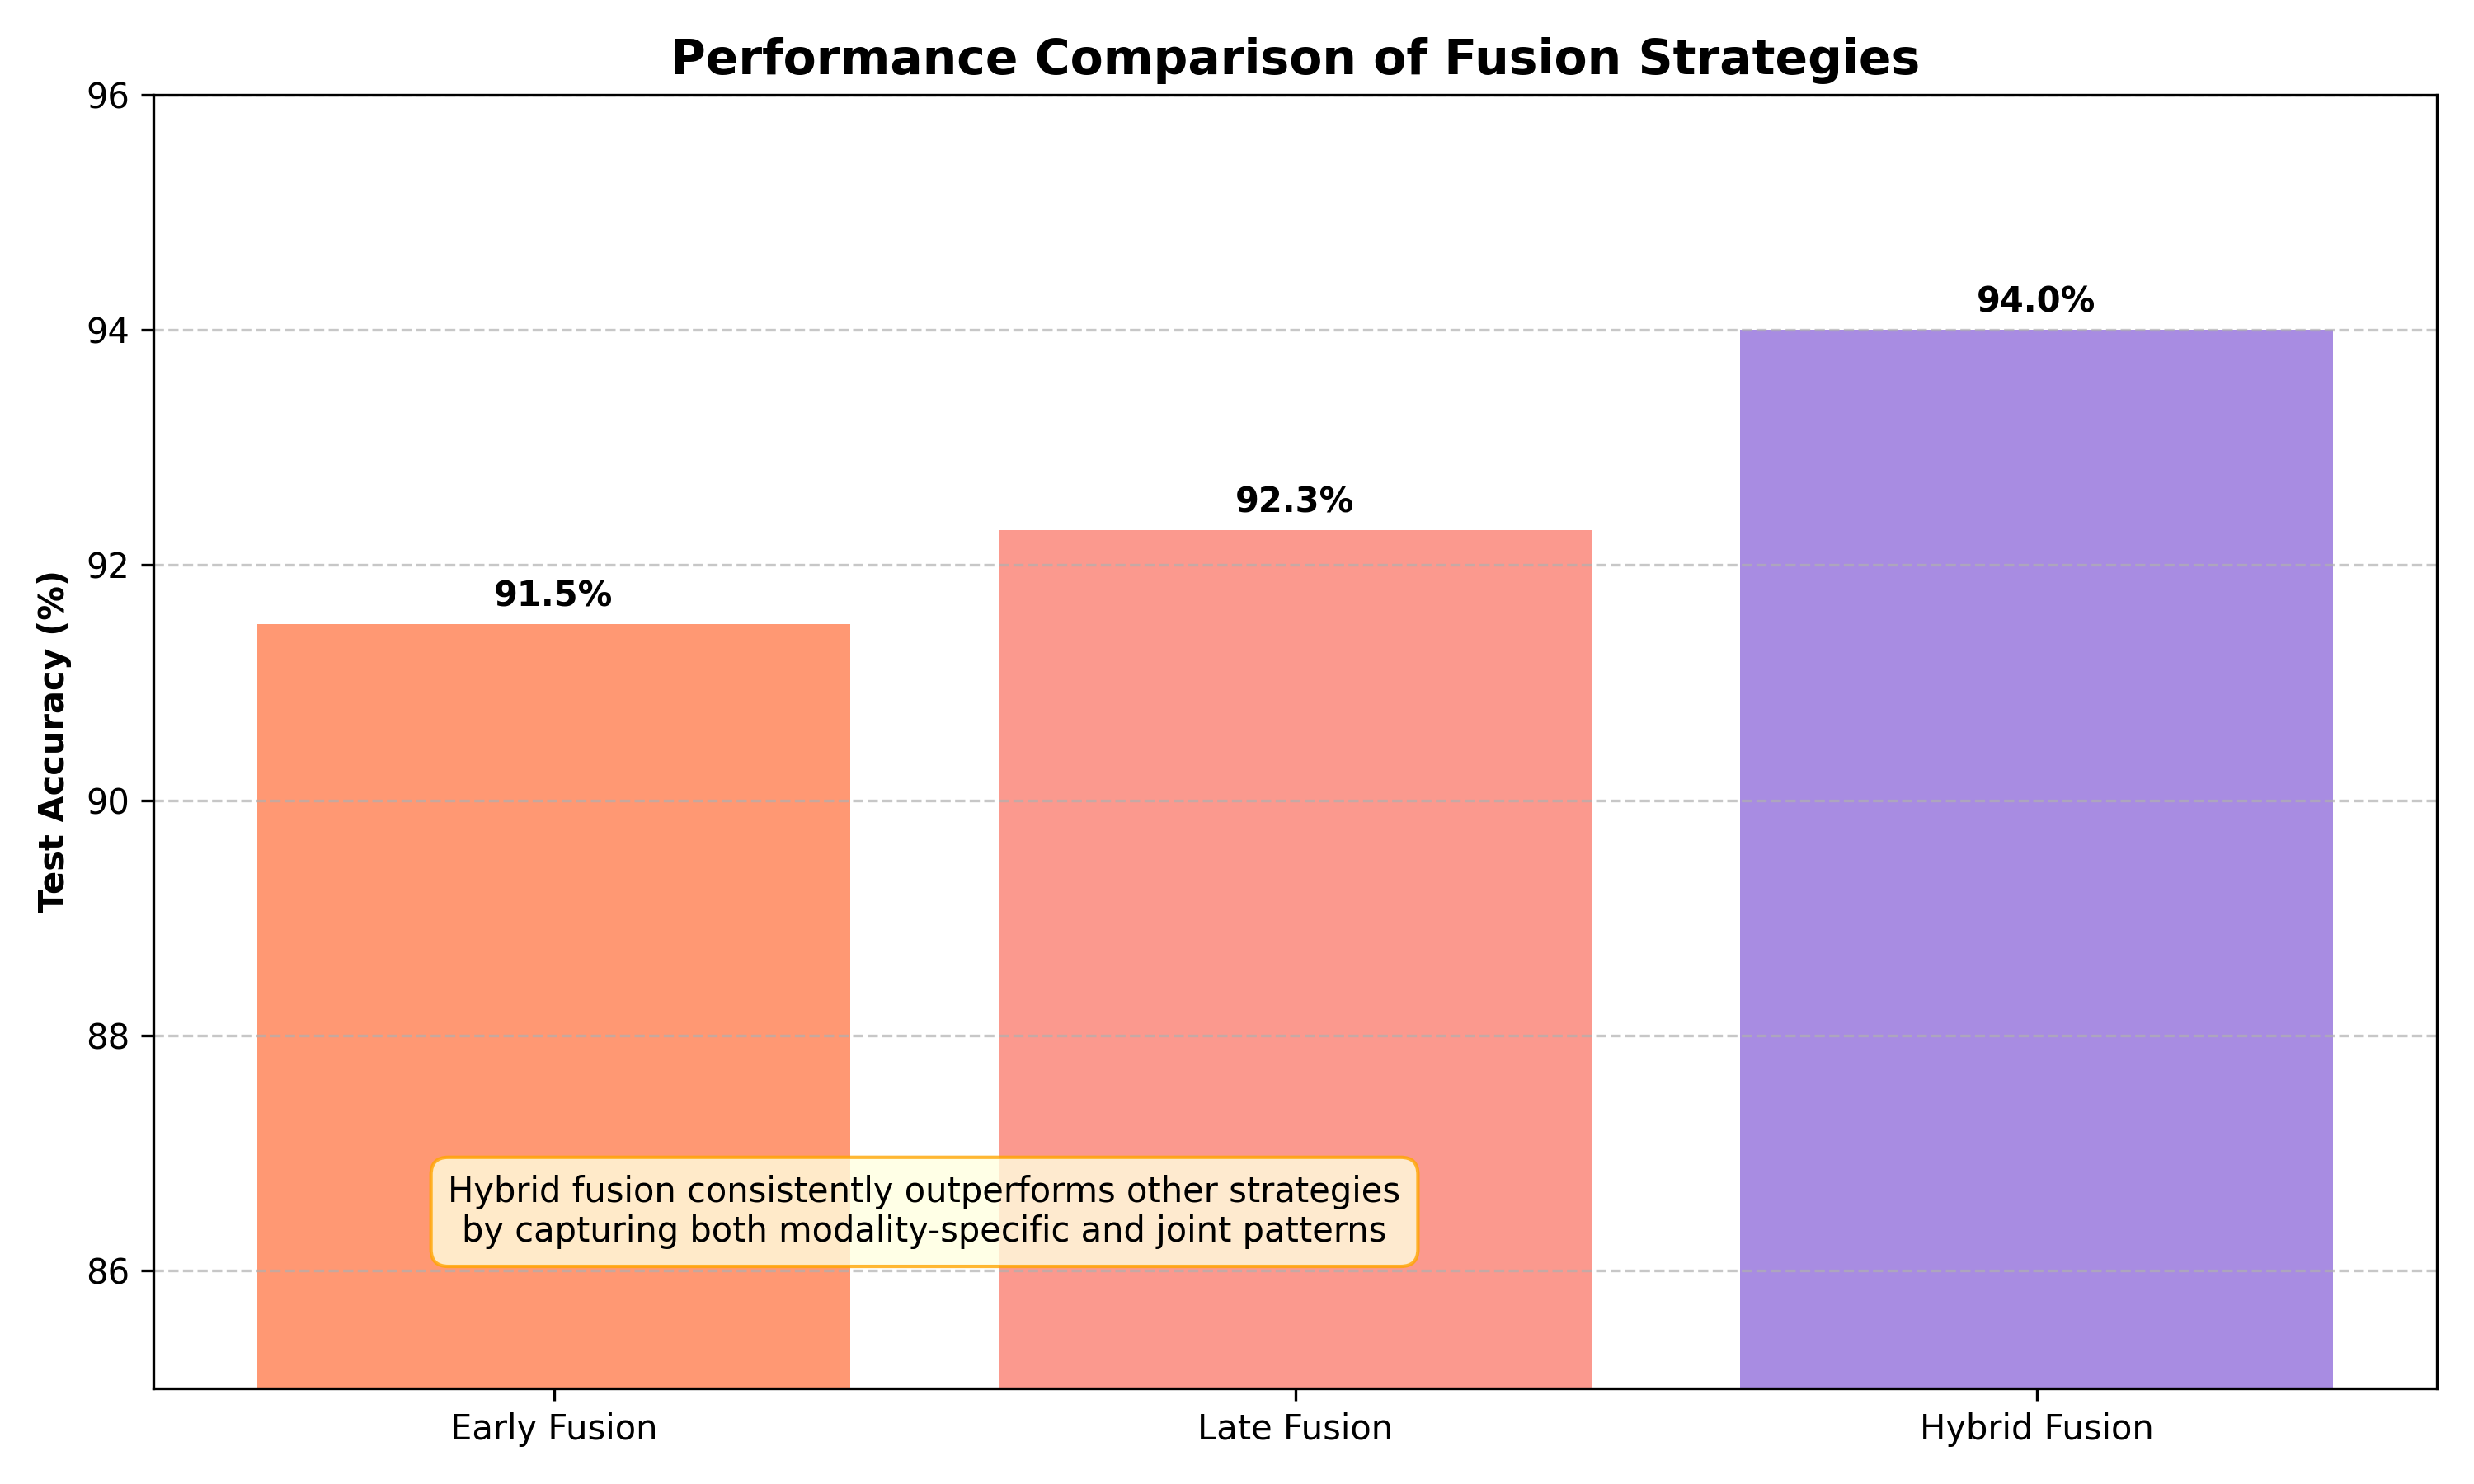
\includegraphics[width=0.9\textwidth]{figures/fusion_performance.png}
\caption{Performance comparison of fusion strategies}
\end{center}

\begin{itemize}
    \item Attention-based fusion provides best overall performance
    \item Late fusion performs well for categorical classification
    \item Early fusion shows inconsistent results across experiments
    \item Hybrid fusion balances performance and computational efficiency
\end{itemize}
\end{frame}

\begin{frame}
\frametitle{Performance-Efficiency Tradeoffs}
\begin{center}
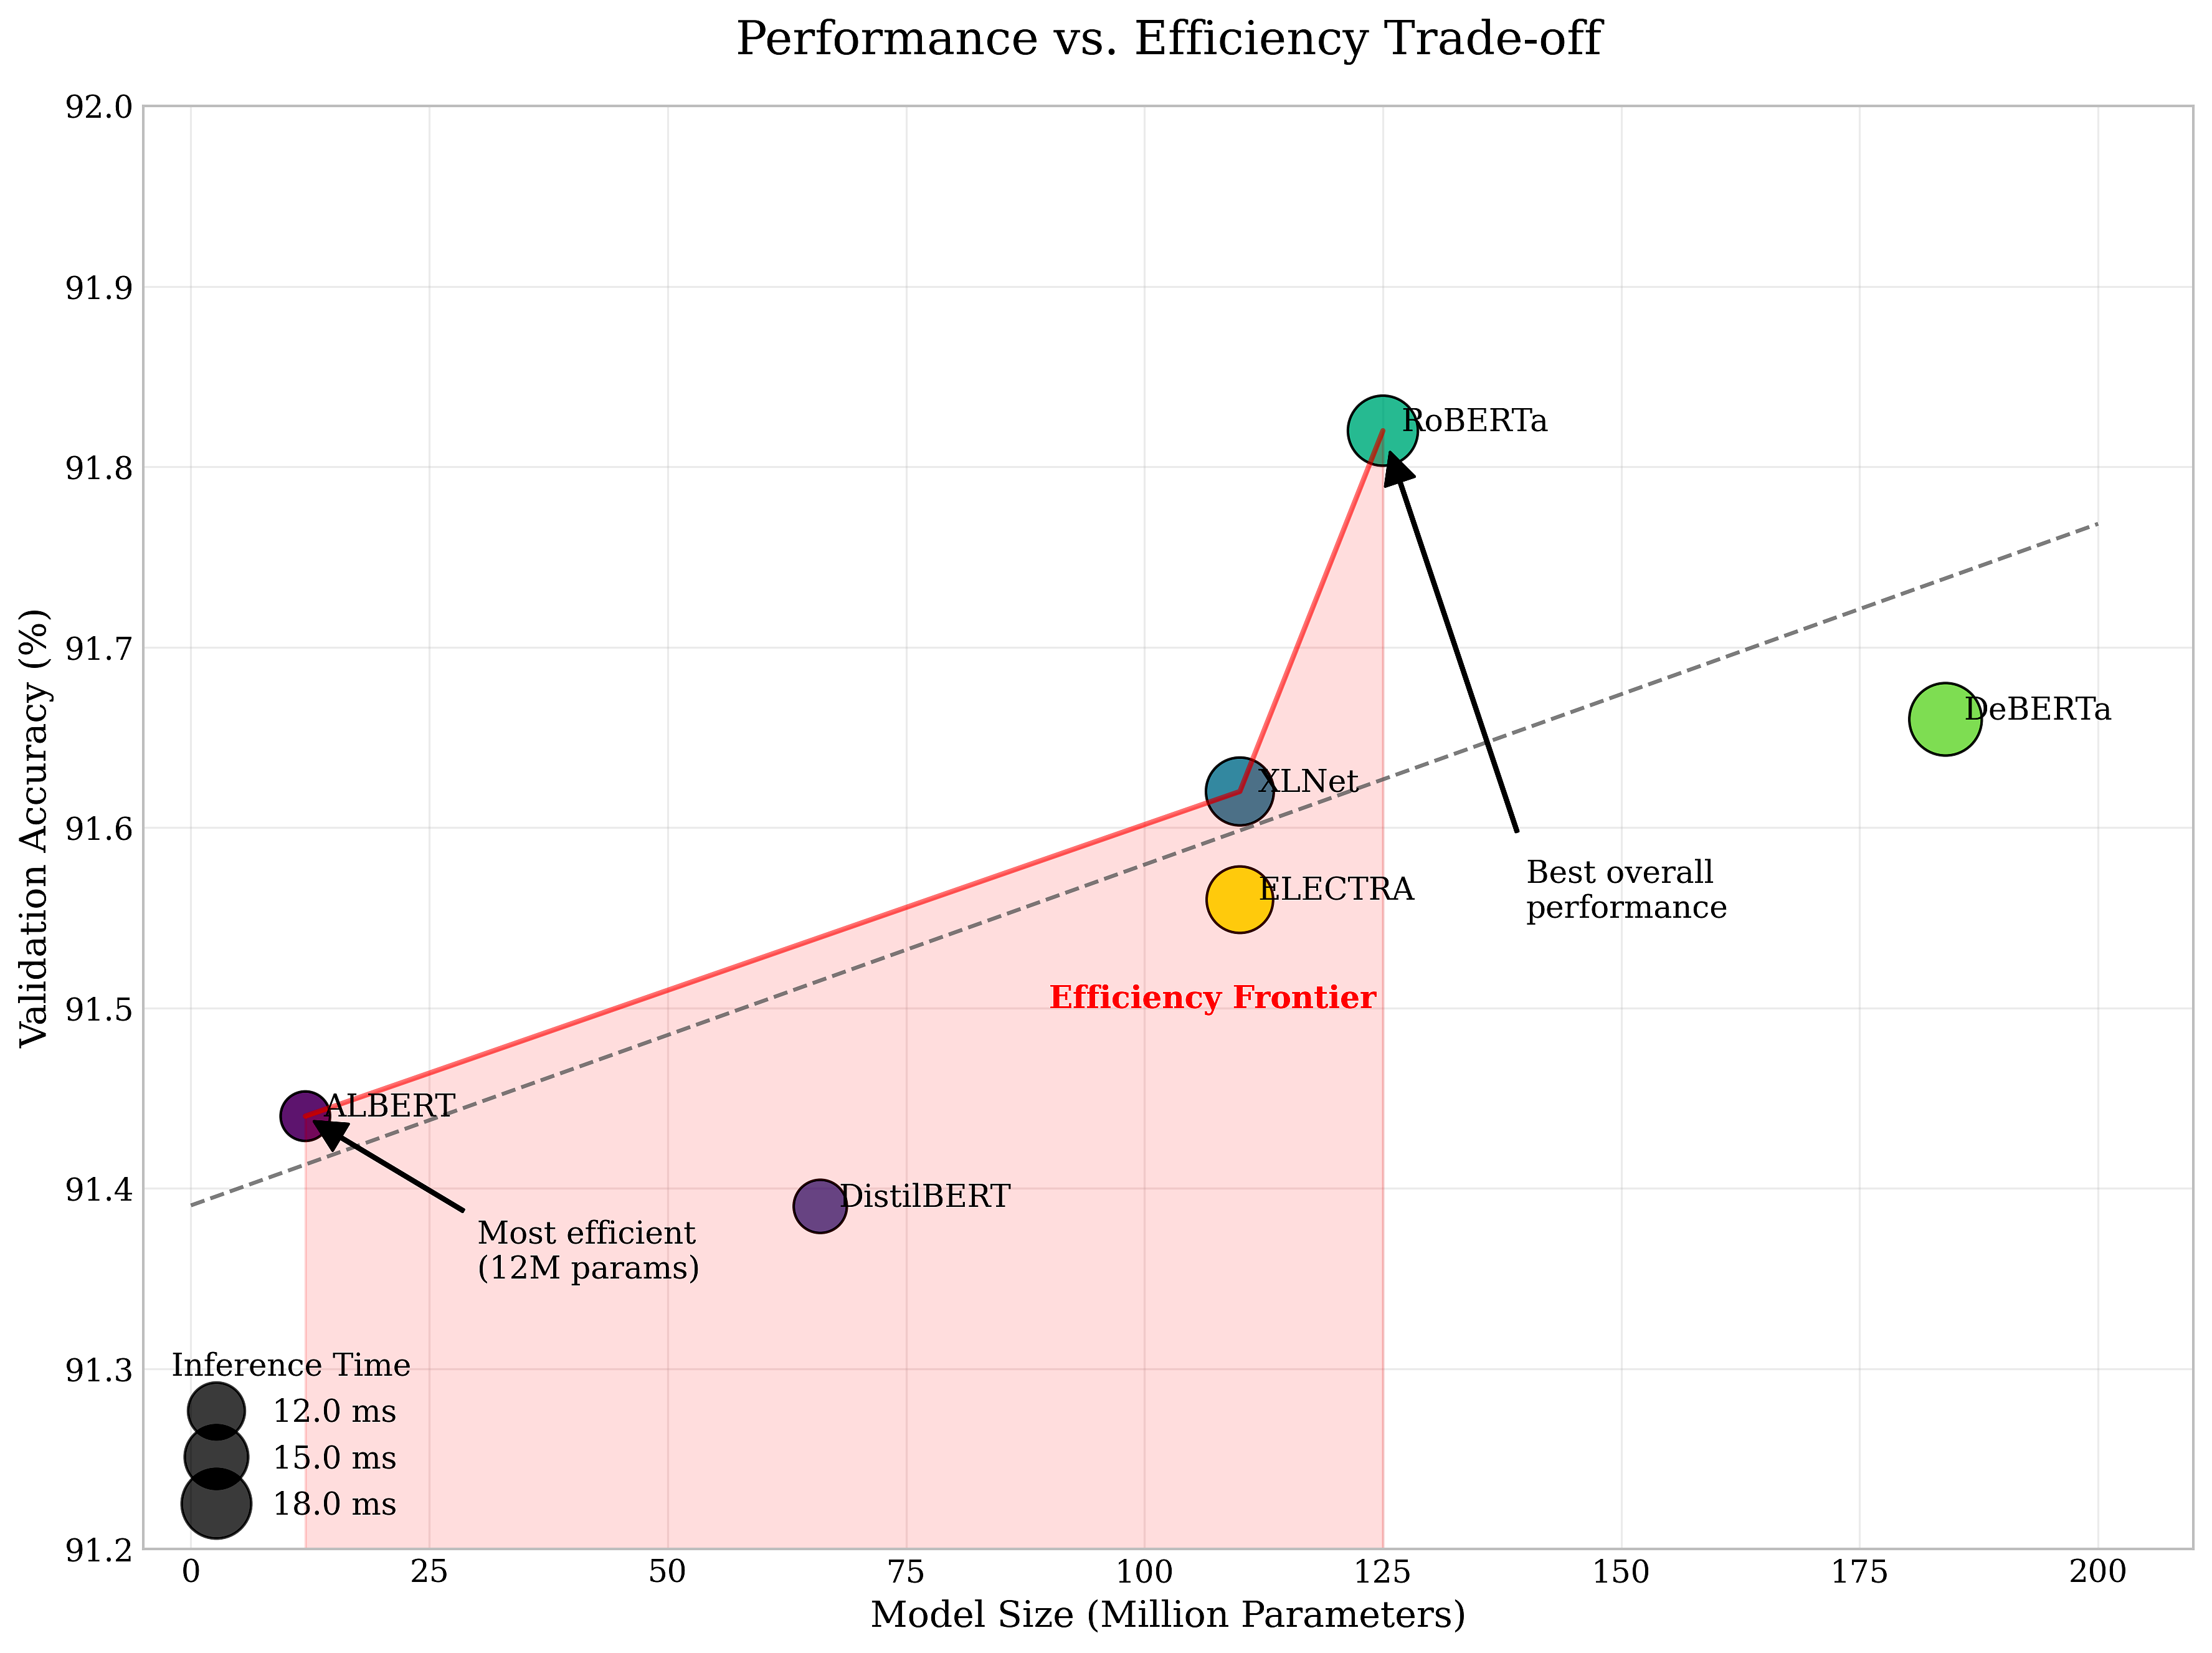
\includegraphics[width=0.9\textwidth]{figures/performance_efficiency.png}
\caption{Performance vs. computational complexity}
\end{center}

\begin{itemize}
    \item RoBERTa provides best performance but higher computational cost
    \item ALBERT offers efficient alternative with moderate performance
    \item Text-only models offer better efficiency than multimodal approaches
    \item Hybrid fusion balances performance and efficiency
\end{itemize}
\end{frame}

\section{Conclusions}

\begin{frame}
\frametitle{Key Findings}
\begin{itemize}
    \item Direct classification slightly outperforms two-stage approach for categorical emotion recognition
    \item Text-only approaches slightly outperform multimodal ones, though the gap narrows with optimal fusion
    \item Textual features better capture valence, while audio features more effectively represent arousal
    \item RoBERTa consistently outperforms other transformer models
    \item Attention-based fusion provides the best integration of multimodal information
\end{itemize}
\end{frame}

\begin{frame}
\frametitle{Practical Implications}
\begin{itemize}
    \item \textbf{Application-Specific Approach Selection}:
    \begin{itemize}
        \item Direct classification: When accuracy is critical
        \item Two-stage approach: When continuous emotional representation is valuable
    \end{itemize}
    \item \textbf{Resource Considerations}:
    \begin{itemize}
        \item Text-only approaches offer better efficiency
        \item ALBERT provides good performance-efficiency tradeoff
    \end{itemize}
    \item \textbf{Modality Selection}:
    \begin{itemize}
        \item Valence-focused applications: Prioritize text
        \item Arousal-focused applications: Incorporate audio
    \end{itemize}
\end{itemize}
\end{frame}

\begin{frame}
\frametitle{Future Work}
\begin{itemize}
    \item Incorporate visual modality (facial expressions, gestures)
    \item Explore more sophisticated fusion techniques (cross-modal attention)
    \item Investigate culture-specific emotional expressions
    \item Develop personalized emotion recognition models
    \item Explore few-shot and zero-shot learning for emotion recognition
    \item Evaluate on more diverse datasets across languages and contexts
\end{itemize}
\end{frame}

\begin{frame}
\frametitle{Thank You}
\begin{center}
\LARGE{Questions?}

\vspace{1cm}
\normalsize
Contact: xiangyi.li@sjsu.edu
\end{center}
\end{frame}

\end{document}